\documentclass[12pt]{mitthesis} 

\usepackage{lgrind, braket, amsmath, paralist,
  amssymb, bbm, booktabs, subfig, color} 

\usepackage[pdftex]{graphicx}
\graphicspath{{figures/}}

\usepackage[version=3]{mhchem}

\newcommand{\TODO} [1]{\textcolor{magenta}{\textbf{TODO:} #1}}
\newcommand{\NOTE} [1]{\textcolor{magenta}{[\emph{#1}]}}
\newcommand{\POINT}[1]{\textcolor{magenta}{\textbf{POINT:} #1}}

\newcommand{\rcm}{cm$^{-1}$}
\newcommand{\bigspace}{$
  \;
  $}

\newcommand{\astate}{$
  \tilde{A} \: ^1\!A_u
  $}
\newcommand{\AtoX}{$
  \tilde{A} \: ^1\!A_u 
  \leftarrow 
  \tilde{X} \: ^1\Sigma_g^+
  $}
\newcommand{\StoS}{$
  S_1 \leftarrow S_0
  $}
\newcommand{\microsec}{$\mu$s}

\newcommand{\Ka}[1]{$K_a\!\!=\!#1$}

% scientific notation
\newcommand{\e}[1]{\ensuremath{\times 10^{#1}}}

% temperatures
\newcommand{\degrees}{\ensuremath{^\circ}}

% hyphenation
\hyphenation{acetylene}
\hyphenation{Hamiltonian}

\begin{document}

\tableofcontents
\clearpage

\listoffigures
\clearpage

\subsubsection*{NOTES}

\clearpage

\setcounter{chapter}{3}
\chapter{SEELEM/LIF spectroscopy of acetylene: Spectral signatures of
  energetically distant doorway levels}

\section{Introduction}

What are the global characteristics of doorway-mediated intersystem
crossing in acetylene, \ce{C2H2}?  Although we have a detailed
understanding of the spectrscopic patterns arising from a crossing
between near-degenerate $S_1$ and $T_3$ vibrational levels
\cite{humphrey97, altunata00, altunata01, mishra04}, we do not know
quite what to anticipate in the spectrum of an $S_1$ level which is
not near-degenerate with a $T_3$ doorway.  In this study, we examine
the spectrum of several $S_1$ vibrational sublevels falling into the
latter category, and produce a cohesive description of
singlet$\sim$triplet mixing that takes into acount the effects of
energetically distant $T_3$ doorway levels.  The spectra of $S_1$
sublevels in this category are far from uneventful, and provide an
unexpected wealth of information as to the nature and relative energy
of $T_3$ vibrational levels.

To observe the distribution of metastable, nominal $T_{1,2,3}$
eigenstates in the vicinity of an allowed $S_1 \leftarrow S_0$
transition, we take advantage of two complementary, simultaneously
recorded spectroscopic detection channels: Laser-Induced Fluorescence
(LIF) and Surface Electron Ejection by Laser-Excited Metastables
(SEELEM).  Gated LIF detection is limited to eigenstates with short
radiative lifetimes ($\tau <$ 10 \microsec), resulting from large
fractional $S_1$ character.  Conversely, SEELEM detection is sensitive
only to long-lived ($\tau >$ 300 \microsec) states with vertical
electronic excitation above an energy threshold determined by the
metal used as the detector surface.  SEELEM detectable eigenstates
must therefore have a small but nonzero amount of fractional $S_1$
character.  As a result, simultaneously recorded LIF and SEELEM
spectra display mutually exclusive sets of eigenstates that arise from
spin-orbit mixed $S_1$ and $T_{3,2,1}$ zero-order basis states.

% Because SEELEM detection is sensitive to the electronic
% character of the molecule, a comparison of simultaneously recorded
% SEELEM and LIF spectra reveals features of electronic structure and
% photochemical pathways that are invisible via traditional,
% single-channel spectroscopic probes such as LIF alone, REMPI,
% phosphorescence, or phosphor surface \cite{shi98, campos01, burton72}.
 
Intersystem crossing in the \astate\ ($S_1$) state of acetylene is
well-described by a doorway-mediated coupling model.  The model is
supported by observations in Zeeman anticrossing spectroscopy
\cite{dupre91, dupre95a, dupre95b}, LIF Zeeman quantum beat
spectroscopy \cite{ochi87, ochi91, dupre93}, high-resolution LIF
spectroscopy \cite{drabbels94, altunata01}, simultaneous LIF and
SEELEM spectroscopy \cite{humphrey97, altunata00, mishra04}, and
photodissociation plus H-atom action spectroscopy \cite{yamakita03,
  loffler98, mordaunt98}.  Briefly, the model states that matrix
elements between vibrational levels of the $S_1$ and $T_{1,2}$
electronic states are very nearly zero, and that all mixing between
$S_1$ and $T_{1,2}$ levels is induced indirectly by nonzero $S_1 \sim
T_3$ and $T_3 \sim T_{1,2}$ matrix elements.

% The
% results of \emph{ab initio} calculations indicate that the electronic
% spin-orbit matrix element is an order of magnitude larger for $S_1
% \sim T_3$ than for $S_1 \sim T_1$.  This result, in combination with
% smaller vibrational overlap integrals resulting from a $\sim$ 10,000
% \rcm\ excess of vibrational energy in the $T_{1,2}$ electronic states,
% accounts for the relative magnitude of the matrix elements according
% to the model.

% Theoretical and experimental
% work confirmed that the coupling doorways were vibrational levels of
% the $T_3$ electronic state \cite{vacek96, sherrill96, humphrey97,
%   altunata00}.

The \emph{trans}-bending mode of $S_1$ acetylene, $\nu_3$, is known to
be an important promoter of $S_1 \sim T_3$ mixing.  In Zeeman
anticrossing experiments, Dupr\'{e} and coworkers observed a rapid
increase in the anticrossing density, as well as the product
$\rho_{\text{vib}} \braket{H_{st}}$, with energy in $\nu_3$
\cite{dupre91, dupre95b}.  They also observed an single large
singlet$\sim$triplet anticrossing in the $3 \nu_3$ $K_a=0$ level,
%with a zero-field matrix element of 0.29 \rcm,
which was in turn perturbed by many smaller couplings \cite{dupre93}.
These observations led the authors to propose that mixing between
$S_1$ and the dense manifold of optically dark states, including
$T_{1,2}$ levels, is controlled by the magnitude of vibrational
overlap factors between $S_1$ levels and particular doorway
vibrational levels.  Subsequent theoretical and experimental work
identified the doorways as vibrational levels of the $T_3$ electronic
state \cite{vacek96, sherrill96, humphrey97, altunata00}.

% best described by a doorway-mediated mechanism, in which particular
% triplet vibrational levels mediate intersystem crossing between the
% initially excited $S_1$ bright state and the dense manifold of highly
% mixed, dark $T_{1,2}$ states.

The $S_1$ $3 \nu_3$ \Ka{1} level has been heavily studied due to the
presence of a near-degenerate vibrational level of $T_3$, which gives
rise to an $S_1 \sim T_3$ level crossing at $J \approx 3$.
Spectroscopic patterns in LIF and SEELEM arising from the effects of
the local $T_3$ perturber are discussed by several authors
\cite{humphrey97, altunata00, altunata01, mishra04}.  Using
vibrational overlap integrals gained from \emph{ab initio}
calculations of the $T_3$ electronic surface, Thom and coauthors were
able to exclude all but several candidate $T_3$ levels as the $3\nu_3$
local perturber \cite{thom07}.
% \POINT{Overlap between $S_1$ and $T_3$ levels predicted by Bryan and
%   Ryan.  (See p.40 of 1/2007--3/2007 notebook.)}
However, a recent observation of increased average $T_{1,2}$
electronic character at $J'=8-12$ suggests that the local $T_3$
perturber is not the sole, and perhaps not the primary, doorway for $3
\nu_3$ \Ka{1} \cite{degroot07}.

That an energetically distant $T_3$ doorway, which would be required
to have a correspondingly larger spin-orbit matrix element, may play a
role in coupling $S_1$ $3 \nu_3$ to the $T_{1,2}$ manifold is not
altogether surprising, given the energy region in question.  \emph{Ab
  initio} calculations are in agreement that an electronic surface
crossing between the $S_1$ and $T_3$ states is energetically nearby
\cite{ventura03, thom07}.  Such a surface crossing would allow for
strong interactions with several $T_3$ levels in the same energy
region.  It should also play a role in promoting singlet$\sim$triplet
coupling within other $S_1$ levels in the same energy region.  The
$4\nu_3$ level, 1000 \rcm\ higher in energy, is also strongly coupled
to the $T_{1,2}$ manifold, although no obvious local $T_3$ doorway has
been observed \cite{drabbels94, ochi91}.  

% The energies of the $3
% \nu_3$ and $4\nu_3$ levels can therefore be taken as conservative
% lower and upper bounds for an ``active'' $S_1 \sim T_3$ coupling
% region.

We turn our attention to other vibrational levels of $S_1$ in the same
energy region that are not near-degenerate with a mediating $T_3$
level at low $J$.  In the absence of a local $T_3$ perturber, coupling
between $S_1$ levels and the local manifold of $T_{1,2}$ levels is
expected to be mediated by energetically distant $T_3$ levels.

% Evidence for energetically distant, mediating $T_3$ levels is obtained
% by comparing simultaneously recorded LIF and SEELEM spectra.

We begin by deriving the energy level spacings and spin-orbit matrix
elements, in general, between vibrational levels of $S_1$ and $T_3$.
Next, we develop a new analysis technique that is sensitive to the
presence of distant $T_3$ doorway levels.  This new technique takes
into account shifting relative intensities in the frequency-domain LIF
spectrum as a function of delay time, which result from the time
development of an incoherent ensemble of eigenstates with different
radiative lifetimes.  We then apply the new technique to the
simultaneous LIF and SEELEM spectra of four $S_1$ vibrational
sublevels, and discuss the properties of admixed, energetically
distant $T_3$ vibrational levels.

\section{Theory: $S_1 \sim T_3$ rotational energy level spacing and
  spin-orbit matrix elements}
\label{theory1}

In the $S_1$ (\astate) electronic state, acetylene is a near-symmetric
prolate top.  Neglecting centrifugal and asymmetry terms, the
rovibrational energies are approximately \cite{watson82}
\begin{equation}
  \label{eq:s1-energy-levels}
  E_{S_1}(v,K,J) = T_v + [A_v - B_v] K^2 + B_v \, J(J+1),
\end{equation}
where $J$ is the total angular momentum, $K$ is the absolute value of
the projection of the orbital angular momentum on the a-axis of the
molecule, $T_v$ is the rotationless energy of the vibrational level
$v$, and $A_v$, $B_v$, and $C_v$ ($\approx B_v$) are the rotational
constants for the vibrational level.  The model of a near-symmetric
prolate top is also appropriate to describe the energy levels of the
$T_3$ electronic state, although \emph{ab initio} calculations predict
that the \emph{trans}-bent equilibrium geometry is non-planar and
therefore slightly more asymmetric \cite{ventura03, thom07}.  Adopting
a Hund's case ($b$) basis, the rovibrational energy levels of $T_3$
are approximately
\begin{equation}
  \label{eq:t3-energy-levels}
  E_{T_3}(v,K,N) = T_v + [A_v - B_v] K^2 + B_v \, N(N+1),
\end{equation}
where the pattern-forming rotational quantum number, $N$, is the total
angular momentum exclusive of spin.  At each energy $E_{T_3}(v,K,N)$,
three near-degenerate spin components are present, due to the three
possible values of the total angular momentum $J$.  The components are
labeled $F_1$ ($J=N+1$), $F_2$ ($J=N$), and $F_3$ ($J=N-1$).  Figure
\ref{fig:triplet-rot-structure} shows an example of the rotational
energy level structure.  Since $S=0$ for the $S_1$ electronic state,
only one component $N=J$ is present for all $S_1$ rotational levels.

The $S_1$ and $T_3$ electronic states are mixed by spin-orbit
interaction.  The total first-order spin-orbit matrix element between
rovibrational states of $S_1$ and $T_3$ is the product of three
factors: an electronic spin-orbit matrix element, a vibrational
overlap factor, and a rotational factor arising from angular momentum
coupling.  Spin-orbit matrix elements follow the rotational selection
rules $\Delta J = 0$ and $\Delta P = 0$, where $P$ is the projection
of $J$ on the a-axis of the molecule \cite{hougen64}.  In Hund's case
($b$), the quantum number $P$ is mixed among several levels with
different $K$, leading to the case ($b$) selection rule $\Delta K = 0,
\pm 1$ \cite{hougen64, stevens73}.

We consider the relative rotational energy differences between an
$S_1$ vibrational sublevel $\ket{S}$ and a $T_3$ vibrational sublevel
$\ket{T}$.  According to the selection rule $\Delta J = 0$, a
rotational level of $\ket{S}$, $\ket{S;J=J_S}$, may mix with three
rotational levels of $\ket{T}$: $\ket{T;N=J_S-1}$ (an $F_1$
component), $\ket{T;N=J_S}$ (an $F_2$ component), and
$\ket{T;N=J_S+1}$ (an $F_3$ component).  Since the three triplet
components with nonzero matrix element differ in the rotational
pattern-forming quantum number, $N$, they have different rotational
energies.  Written in terms of $J$, these energies are
\begin{equation}
  E_T(J) = T_{0,T} + 
  \begin{cases}
    B_T \, (J+1)(J+2) & F_3 \:\: (\Delta N = +1), \\
    B_T \, J(J+1)     & F_2 \:\: (\Delta N = 0), \\
    B_T \, J(J-1)     & F_1 \:\: (\Delta N = -1),
  \end{cases}
\end{equation}
where $T_{0,T}$ is the rotationless energy of $\ket{T}$.  Subtracting
the rotational energies of $\ket{S}$,
\begin{equation}
  E_S(J) = T_{0,S} + B_S \, J(J+1),
\end{equation}
from $E_T(J)$ yields the rotational energy differences between
$\ket{S}$ and $\ket{T}$.  In the approximation that the difference in
rotational constants $\Delta B_{ST}$ is small compared to $B_T$, the
rotational energy differences are
\begin{equation}
  \label{eq:components}
  \Delta E_{ST}(J) = \Delta T_0 +
  \begin{cases}
    \:\: 2B_TJ + 2 B_T 
    & F_3 \:\: (\Delta N = +1), \\
    \:\: 0
    & F_2 \:\: (\Delta N = 0), \\
    \:\: - 2B_TJ
    & F_1 \:\: (\Delta N = -1).
  \end{cases}
\end{equation}

\begin{figure}
  \caption{\TODO{Write caption} }
  \label{fig:rotational-energy-differences}
  \centering
  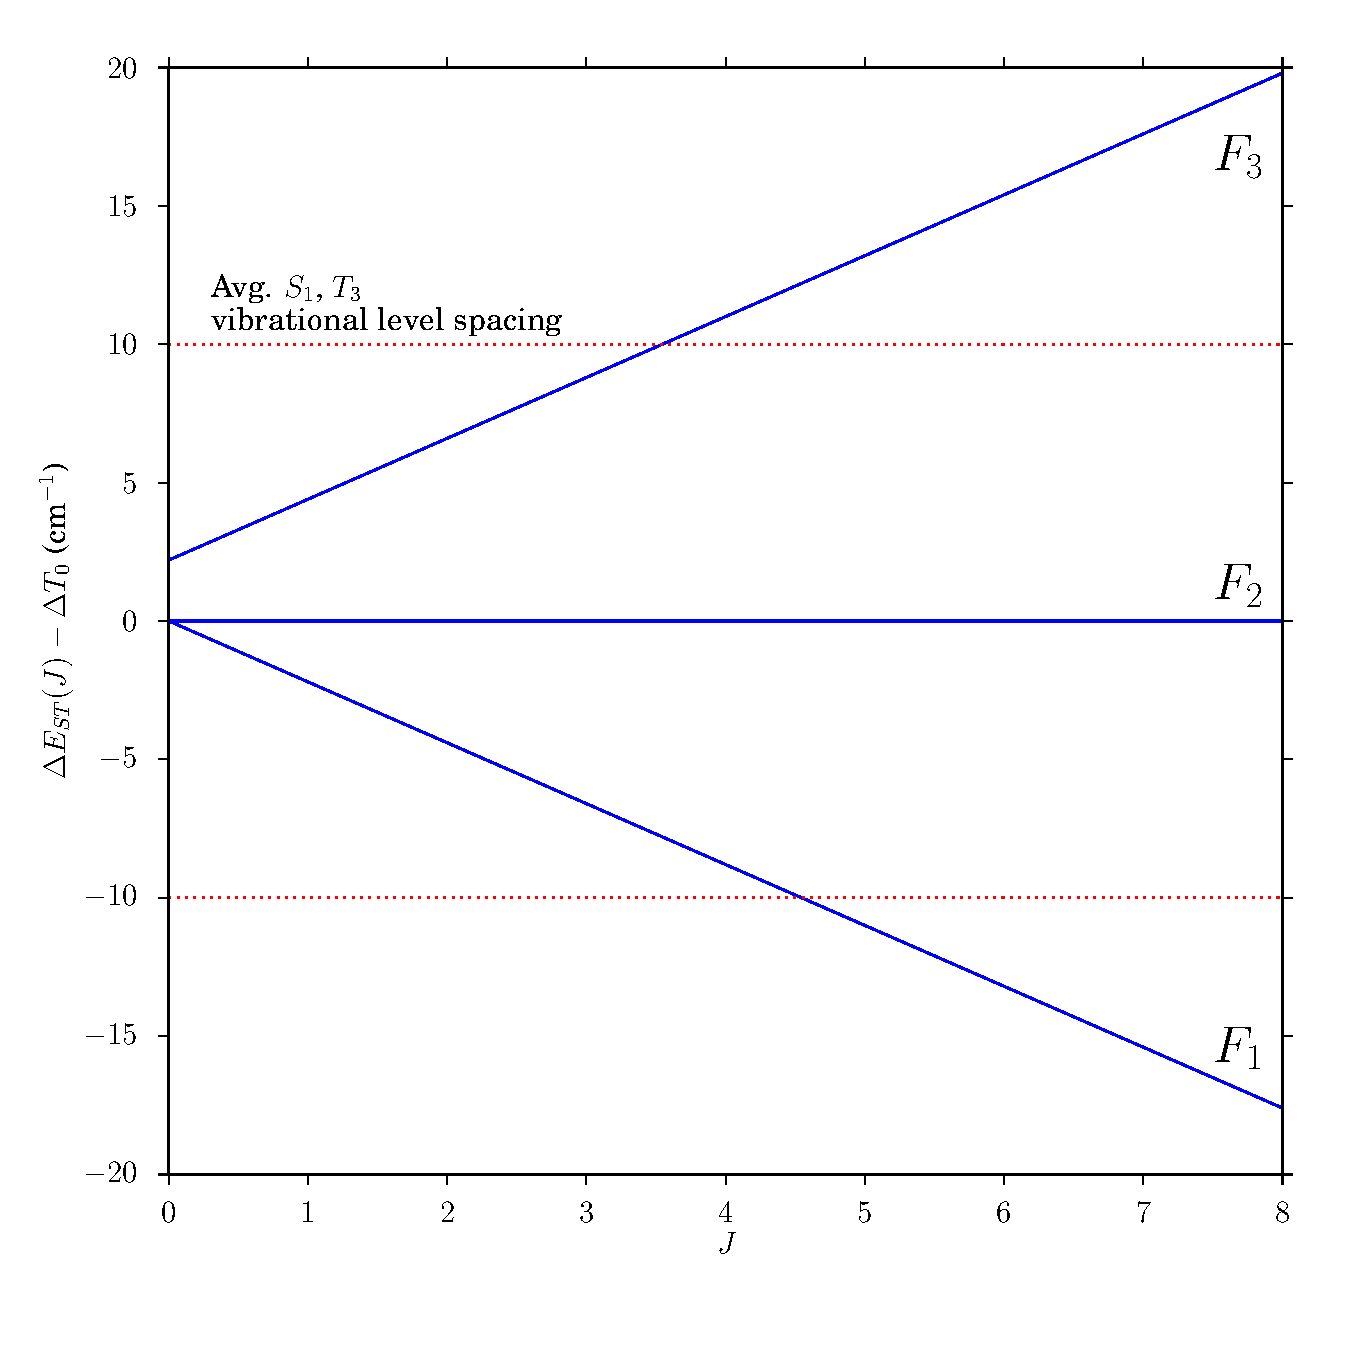
\includegraphics[width=6in]{rotational-energy-differences.pdf}
\end{figure}

The approximate energy differences $\Delta E_{ST}(J)$ are plotted as a
function of $J$ in Figure \ref{fig:rotational-energy-differences}.  A
value of $B_T=1.1$ \rcm\ was chosen for the figure based on the
rotational assignment of a $T_3$ perturber in the $3^3$ \Ka{1}
sublevel of $S_1$ \cite{mishra04}.  The relative energy of the $F_2$
component has a slope of approximately zero, while the relative
energies of the $F_1$ and $F_3$ components have slopes of
approximately $-2B_T \approx -2$ \rcm\ and $+2B_T \approx +2$ \rcm\
per $J$, respectively.  Also included on the plot is the average
vibrational level spacing $\rho^{-1} \approx 10$ \rcm\ for both the
$S_1$ and $T_3$ electronic states.  The relative energies of the $F_1$
and $F_2$ components are 10 \rcm\ distant from their initial positions
when $J \approx 4$.

Because the $F_1$ and $F_3$ components of the triplet have large
slopes in relative energy spearation from a singlet level, the
component of a $T_3$ level with which an $S_1$ level interacts is
determined by the rotationless energy difference.  The possibilites
are as follows.
\begin{itemize}
\item When two vibrational sublevels of $S_1$ and $T_3$ are
  near-degenerate, $-4 \lesssim (T_{0,T} - T_{0,S}) \lesssim 2$ \rcm,
  the energy separation between the singlet and the $F_2$ component of
  the triplet remains close to its initial value as $J$ increases,
  while the relative energy separations of the $F_1$ and $F_2$
  components increase at a rate of approximately $2B_T$ per $J$.
  Energy denominators favor mixing between the singlet and the $F_2$
  component of the triplet when $J \ge 1$.
\item When a $T_3$ doorway level lies higher in rotationless energy
  than the singlet level, $ (T_{0,T} - T_{0,S}) \gtrsim 2$ \rcm,
  energy denominators favor mixing between the singlet and the $F_1$
  component of the triplet.  The rotational energy separation between
  the singlet and the $F_1$ component of the triplet decreases at a
  rate of approximately $2B_T$ per $J$ until a level crossing occurs
  at $J \approx (T_{0,T} - T_{0,S}) / 2 B_T$.
\item When a $T_3$ doorway level lies below a singlet level in
  rotationless energy, $(T_{0,T} - T_{0,S}) \lesssim 4$ \rcm, energy
  denominators determine that the primary interaction is via the
  triplet $F_3$ component.  The rotational energy separation between
  the singlet level and the $F_3$ component of the triplet decreases
  at a rate of $2B_T$ per $J$ until a crossing occurs at $J \approx
  (T_{0,S} - T_{0,T}) / 2 B_T - 1$.
\end{itemize}
Taken together, these trends guarantee a level crossing at $J<8$ for
any pair of $S_1$ and $T_3$ sublevels having a rotationless energy
separation of less than 20 \rcm.  Regardless of the sign of the
rotationless energy difference, one spin component of a $T_3$ level
always approaches the singlet in rotational energy separation at a
rate of $2B_T$ per $J$.  When a doorway is energetically distant, in
other words not near-degenerate in rotationless energy, energy
denominators determine that the interaction occurs via either the
$F_1$ or $F_3$ component, depending on the sign of $T_{0,T} - T_{0,S}$.

\begin{figure}[p]
  \caption{Rotational factors of spin-orbit matrix elements between
    rovibrational levels of the $S_1$ and $T_3$ electronic states,
    $K_S$=1.  The plot includes matrix elements for the $F_3$ ($\Delta
    N = +1$) and $F_1$ ($\Delta N = -1$) components of a $T_3$
    sublevel with $K_T=0,1,2$.  The rotational factors deviate in all
    cases by less than a factor of 2 from their initial positions as a
    function of $J$.}
  \label{fig:rotational-factors-1}
  \centering
  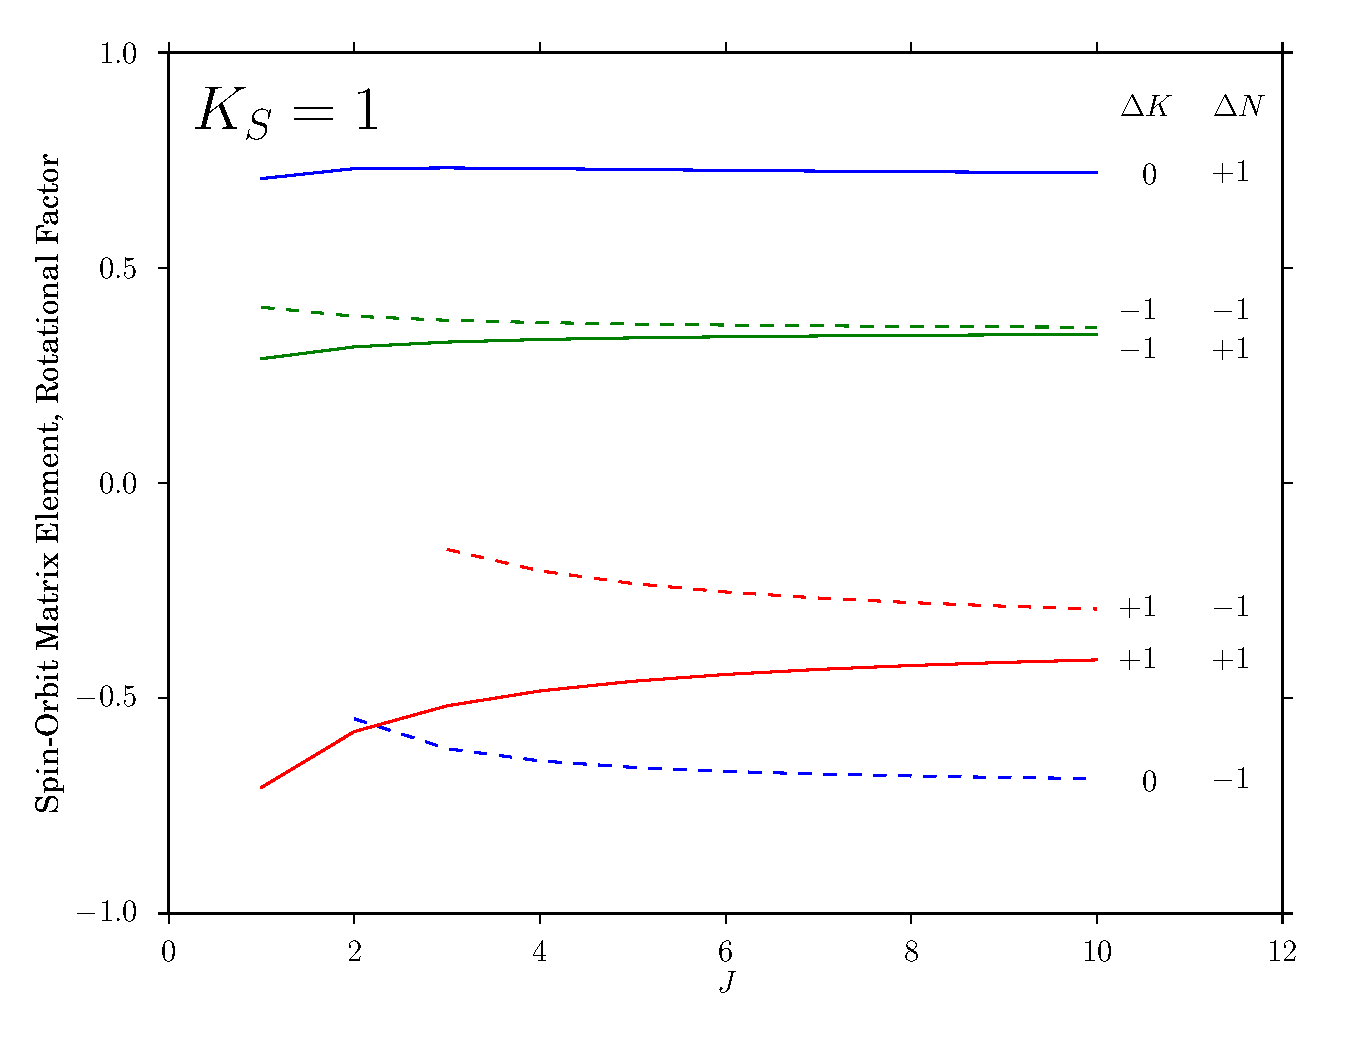
\includegraphics[width=6in]{rotational-factors-k1.pdf}
\end{figure}

\begin{figure}[p]
  \caption{Rotational factors of spin-orbit matrix elements between
    rovibrational levels of the $S_1$ and $T_3$ electronic states,
    $K_S$=2.  The plot includes matrix elements for the $F_3$ ($\Delta
    N = +1$) and $F_1$ ($\Delta N = -1$) components of a $T_3$
    sublevel with $K_T=1,2,3$.  The rotational factors are essentially
    the same as those for $K_S=1$.}
  \label{fig:rotational-factors-2}
  \centering
  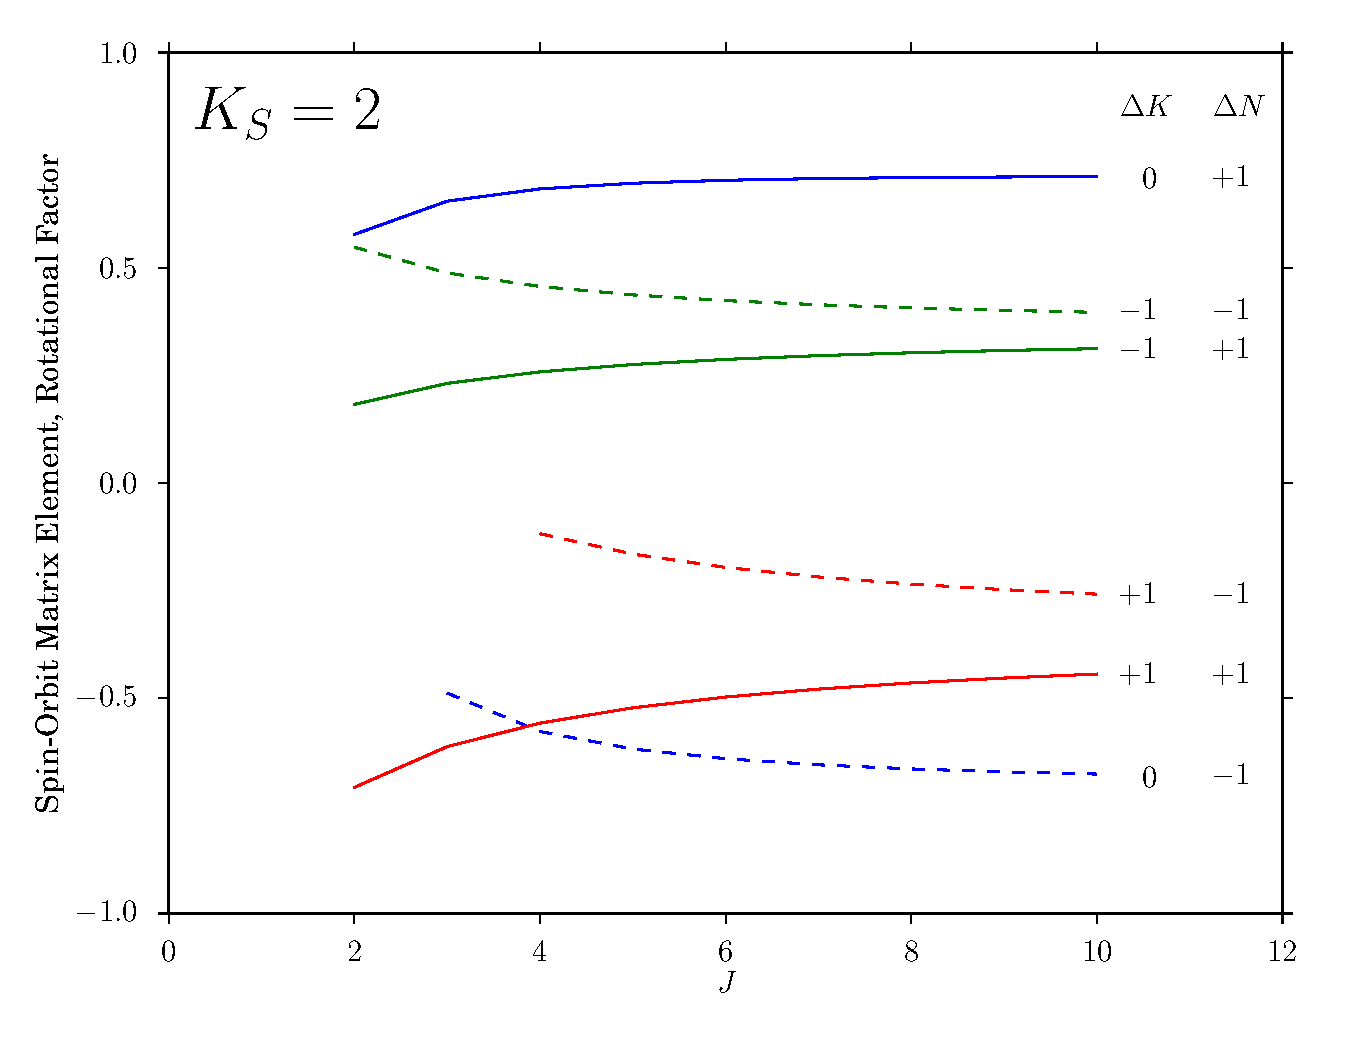
\includegraphics[width=6in]{rotational-factors-k2.pdf}
\end{figure}

To verify that the magnitude of the spin-orbit matrix elements does
not dominate over energy denominator effects for the $F_1$ and $F_3$
components of a triplet level, the rotational factors for spin-orbit
matrix elements were calculated from general formulas given by Stevens
and Brand \cite{stevens73}.  These factors are plotted as a function
of $J$ in Figure \ref{fig:rotational-factors-1} for a singlet level
with $K_S$=1.  The rotational factors quickly approach their
asymptotic limits as $J$ is increased.  Even at low $J$, the
rotational factor never differs from its asymptotic value by more than
a factor of 2.  Figure \ref{fig:rotational-factors-2} shows the same
factors for $K_S$=2, also considered in this study.  The plot is
essentially the same.

The overall magnitude of spin-orbit matrix elements between
rovibrational levels of $S_1$ and $T_3$ is therefore not governed by
rotational factors, but by vibrational overlap factors.  Franck-Condon
overlap between relatively low-lying vibrational levels of $S_1$ and
$T_3$ is calculated to vary over at least three orders of magnitude
\cite{thom07}.  The wide variation in spin-orbit matrix element,
arising from vibrational overlap factors, gives rise to two classes of
level crossings between non-near-degenerate $S_1$ and $T_3$ levels:
those where $H_{ST}^2 \ll 2B_T$, and those where $H_{ST}^2$ is on the
order of $2B_T$.

When $H_{ST}^2 \ll 2B_T$, energy denominator effects cause an $S_1
\sim T_3$ level crossing to be observable at only one $J$ in the
spectrum.  However, once a triplet level with small vibrational
overlap is found at a particular $J$, its energy above or below the
perturbed singlet level may be found according to Equation
\ref{eq:components}.  If the rotationless energy of the triplet
vibrational level is higher than that of the singlet, the triplet must
have $T_{0,T} \approx T_{0,S} + 2B_TJ$.  If the rotationless energy of
the triplet vibrational level is lower than that of the singlet, the
triplet must have $T_{0,T} \approx T_{0,S} - 2B_TJ - 2B_T$.

When $H_{ST}^2$ is on the order of $2B_T$, significant mixing between
the $S_1$ and $T_3$ levels may occur at several consecutive values of
$J$.  Such $T_3$ levels, having $H_{ST}^2$ on the order of $2B_T$, and
lying more than $4B_T$ away in rotationless energy, are the
energetically distant doorway states with which we are most concerned.
By first mixing with the $T_3$ level, the $S_1$ level is permitted to
mix with the local manifold of $T_{1,2}$ levels.  Although a level
crossing with the mediating $T_3$ level may occur too high in $J$ to
be observed, some $T_3$-mediated $S_1 \sim T_{1,2}$ mixing is
observable in the spectrum of the $S_1$ level.  Mixing between the
$S_1$ level and nearby $T_{1,2}$ levels is influenced by the relative
energy of the doorway level: mixing is increased with $T_{1,2}$ levels
that lie closer in energy to the doorway.  In the following section,
we explain this effect and examine a method by which it may be
observed.



























\section{Theory: Signatures of doorway-mediated intersystem crossing
  in delayed, incoherent fluorescence measurements}

An energetically distant $T_3$ doorway level leaves traces of its
presence in the LIF and SEELEM spectra of $S_1$ levels with which it
interacts.  When an $S_1$ level mixes with an energetically distant
$T_3$ doorway level, the relative energy of the doorway has an
influence on the local mixing between the $S_1$ level and nearby
$T_{1,2}$ levels.  This leads to a local energy dependence of the
average fractional $S_1$ character in nominal $T_{1,2}$ eigenstates.
This quantity may be evaluated using perturbation theory, after first
pre-diagonalizing the interaction between $S_1$ and $T_3$.  Following
Chapter 2, Formula 2.4, we find the average fractional $S_1$
character, $\braket{a_{S_1}}^2$, to be
\begin{equation}
  \label{eq:ave-s1-char}
    \braket{a_{S_1}}^2(E) = 
    \alpha^2 (1-\alpha^2) \braket{H_{T_3T_{1,2}}}^2
    \biggl \lbrace 
    \frac{1}{E - E_{S_1}} 
    + \frac{1}{E - E_{T_3}} 
    \biggr \rbrace^2,
\end{equation}
where $\alpha$ is the mixing angle between the $S_1$ level and the
doorway state, $\braket{H_{T_3T_{1,2}}}$ is the average $T_3 \sim
T_{1,2}$ matrix element, $E_{S_1}$ is the energy of the nominal $S_1$
eigenstate and $E_{T_3}$ is the energy of the nominal $T_3$
eigenstate.  

The energy dependence of average fractional $S_1$ character in the
ensemble of nominal $T_{1,2}$ eigenstates causes their
intensity-weighted center of gravity,
\begin{equation}
  \label{eq:cog-def}
  E_{\text{ave}} = \int E \times I(E) \; dE,
\end{equation}
to be offset slightly relative to the energy of the nominal $S_1$
eigenstate in the LIF spectrum.  Since the total fluorescence
intensity of an eigenstate is proportional to its fractional $S_1$
character (see Chapter 3), the magnitude and direction of the center
of gravity offset is found by combining Equations \ref{eq:ave-s1-char}
and \ref{eq:cog-def}:
\begin{equation}
  \begin{split}
    E_{\text{ave}} 
    &= \int E \times \braket{a_{S_1}}^2(E) \; dE,\\
    &= \text{OH NOES WHATS TEH INTEGRALS????!!!1!!11}.
  \end{split}
\end{equation}
We have thus derived the approximate center of gravity offset for an
ensemble of nominal $T_{1,2}$ eigenstates.

As we will demonstrate shortly, the lifetime of the nominal $S_1$
eigenstate is shorter than that of any nominal $T_{1,2}$ eigenstate.
The difference in lifetimes gives rise to changes in the relative
intensity of the $S_1$ eigenstate relative to that of the nominal
$T_{1,2}$ eigenstates as a function of time delay after excitation of
the molecules.  Changes in the relative intensity lead to changes in
the overall center of gravity, when the metric is computed from the
total fluorescence intensity within a delayed time window $t$ to
$t+dt$ after excitation.  In the remainder of this section, we examine
the dependence of the intensity-weighted center-of-gravity on time
delay for an incoherent ensemble of mixed $S_1 \sim T_3$ eigenstates.





\subsection{Characteristics of an incoherent, high-resolution
  fluorescence spectrum after a time delay}

For a pure $S_1$ rovibrational level, $\ket{s}$, the time-dependent
fluorescence intensity is
\begin{equation}
  I_s(t) = \frac{1}{\tau_s} \;
           \exp \left[
             -\frac{t}{ \tau_s} 
           \right],
\end{equation}
normalized such that $\int_0^{\infty} I_s(t) \, dt = 1$.  The quantity
$\tau_s$ is the radiative lifetime of the zero-order $S_1$ level.  In
acetylene, this quantity is largely independent of vibrational and
rotational levels within $S_1$, and is determined to be approximately
270 ns \cite{ochi91, stephenson84}.

We consider the case where $\ket{s}$ is admixed, through an
energetically distant $T_3$ doorway, into $T_{1,2}$ triplet levels to
create a set of singlet$\sim$triplet mixed eigenstates $\lbrace
\ket{m} \rbrace$, each having some fractional $S_1$ character $a_m^2$.
If the lifetime of a pure triplet level is much longer than $\tau_s$,
the lifetime of a mixed eigenstate $\ket{m}$ is
\begin{equation}
  \label{eq:tau-m}
  \tau_m = \tau_s / a_m^2,
\end{equation}
and its time-dependent fluorescence intensity is
\begin{equation}
  \label{eq:int-m}
  I_m(t) = \frac{a_m^4}{\tau_s} \;
           \exp \left[
             -\frac{a_m^2 \, t}{\tau_s} 
           \right].
\end{equation}
The total integrated fluorescence intensity for a mixed state is
$\int_0^{\infty} I_m(t) \, dt = a_m^2$, relative to unit intensity for
a pure $S_1$ state.  This reflects the $a_m^2$ times smaller
probability for excitation of a mixed eigenstate $\ket{m}$.

The relative fluorescence intensity among an incoherent ensemble of
singlet$\sim$triplet mixed eigenstates is examined after a time delay
$t$.  The upper limit of time delay that can be selected in our LIF
experiments is determined by the field-of-view of the fluorescence
detection optics.  In this study, the field-of-view of the
fluorescence detection optics is about 5 mm.  The maximum viewing time
is therefore about about 5 \microsec\ $\approx 18\tau_s$, for
molecules travelling in the molecular beam with average velocity
$\approx 10^3$ m/s.  At a time delay greater than $18\tau_s$, no
molecules remain to be seen within the fluorescence field of view.

At a chosen value of time delay, the relative fluorescence intensity
among an enemble of mixed states has a single maximum with respect to
fractional $S_1$ character, $a_m^2$.  States having the
greatest amount of fractional $S_1$ character fluoresce
quickly.  Although they begin with the greatest intensity, their
relative intensity decreases rapidly with respect to longer-lived
states.  Eigenstates having the smallest amount of fractional bright
state character, conversely, have lesser intensity at $t=0$.  However,
they fluoresce slowly, and as a consequence their relative intensity
increases with time delay, compared to other eigenstates in the
ensemble.

At a given time delay, $t$, the fractional $S_1$ character having the
greatest relative intensity is found by taking the derivative of
eigenstate intensity (Equation \ref{eq:int-m}) with respect to
fractional $S_1$ character, $a_m^2$.  Doing this, we find
\begin{equation}
 \frac{ \partial I_m }{ \partial a_m^2 } =
   \frac{a_m^2}{\tau_s}
   \exp \left[
     -\frac{a_m^2 \, t}{\tau_s} 
   \right]
   \left (
     2 - \frac{a_m^2 \, t}{\tau_s}
   \right ).
\end{equation}
When $t \leq 2\tau_s$, the fluorescence intensity equation increases
monotonically with fractional $S_1$ character, and is maximized
when the fractional $S_1$ character is 1.  When $t > 2 \tau_s$,
the fluorescence intensity equation is at a maximum when the
fractional $S_1$ character is
\begin{equation}
  \label{eq:am-max}
  a_m^2 = \frac{2 \tau_s}{t}.
\end{equation}

\begin{figure}
  \caption{The intensity of a mixed eigenstate at time $R =
    t/\tau_s$, plotted as a function of bright
    state character.}
  \label{fig:int-at-rc}
  \centering
  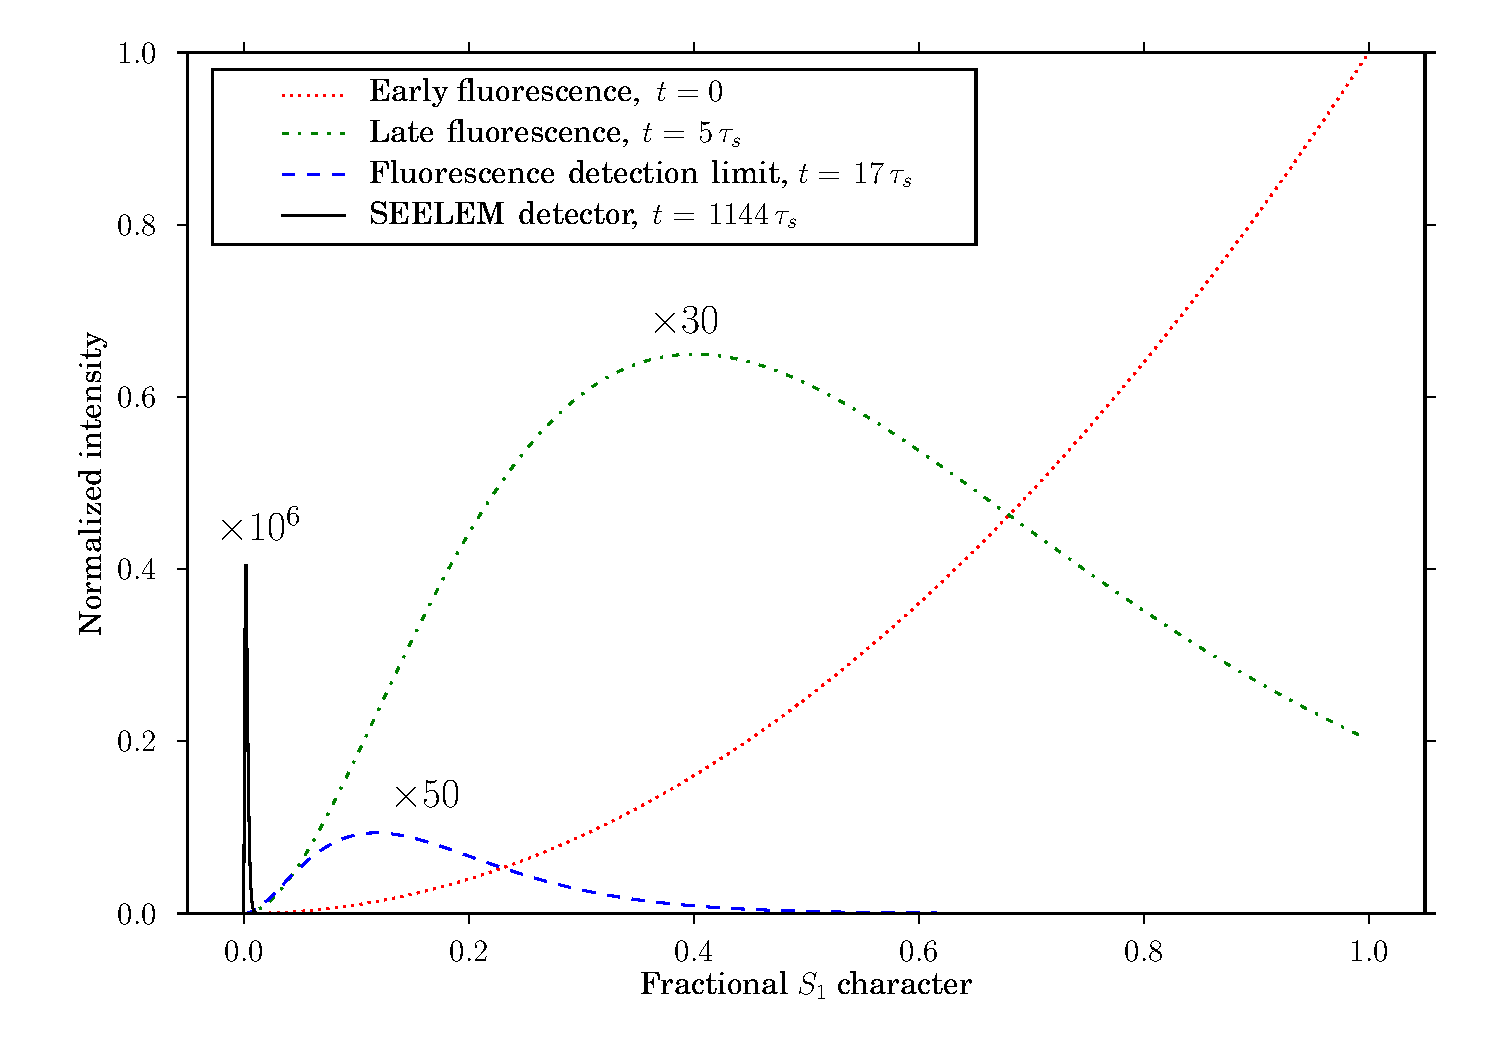
\includegraphics[width=7.5in,angle=90]{intensity-at-delay.pdf}
\end{figure}


Figure \ref{fig:int-at-rc} shows the dependence of fluorescence
intensity on fractional $S_1$ character at several selectable
values of time delay.  When $t = 0$, the fluorescence intensity is
monotonic and greatest for eigenstates containing the greatest amount
of fractional $S_1$ character.  At a delay of $t = 5 \tau_s$,
the fluorescence intensity equation is ``tuned'' to states with a
fractional $S_1$ character of 40\%.  Molecules in eigenstates
containing too much fractional $S_1$ character are
discriminated against, because they have already fluoresced with high
probability by a time delay of $5 \tau_s$.  Molecules in eigenstates
with fractional $S_1$ character $\ll$ 40\% have a low
probability of fluorescing in the time window under consideration, and
are also discriminated against at this delay time.  Figure
\ref{fig:int-at-rc} also shows the dependence of fluorescence
intensity on fractional $S_1$ character for $t=18\tau_s$, the
maximum fluorescence time delay used in this study.  At this time
delay, the fluorescence intensity is peaked at a fractional $S_1$
character of approximately 22\%.

The SEELEM detector used in this study detects metastable acetylene
molecules after a flight time of $\tau_f =$ 309
\microsec.  Considering only the SEELEM electron ejection probability
resulting from $S_1$ electronic character, the total SEELEM detection
probability is (Chapter 2, equation 28):
\begin{equation}
  \label{eq:seelem-prob-s}
  P_{\text{SEELEM}} \propto 
    a_m^4 \; 
    \exp \left [ 
      -\frac{a_m^2 \tau_f}{\tau_s} 
    \right ].
\end{equation}
This is a good approximation to the total SEELEM detection
probability, including electron ejection probability resulting from
fractional $T_3$ electronic character, when a $T_3$ doorway state is
energetically distant (see Chapter 2, section 2.3.2).  The SEELEM
detection probability, Equation \ref{eq:seelem-prob-s}, has the same
functional form as the delayed LIF intensity, Equation \ref{eq:int-m}.
At a flight time of 309 \microsec\, the detection probability is at a
maximum for eigenstates with 0.17\% fractional $S_1$ character.  In
this approximation, the SEELEM detector may be viewed as an extreme
discriminator for detecting states with small fractional $S_1$
character.  The dependence of SEELEM detection probability on
fractional $S_1$ character is also included in Figure
\ref{fig:int-at-rc}.




\subsection{Dependence of the intensity-weighted center of gravity on
  time delay}

Our next step is to examine how the LIF intensity-weighted center of
gravity metric,
\begin{equation}
  E_{\text{ave}} = \int E \times I(E) \; dE,
\end{equation}
changes as the time delay is increased.  We model the interaction
between a rovibrational level of $S_1$ and the local ensemble of
$T_{1,2}$ rovibrational levels by first constructing a model system
containing only one $T_{1,2}$ basis state.


Consider a Hamiltonian containing one $S_1$ level, $\ket{s}$, and one
$T_{1,2}$ level, $\ket{t}$.  Let us define the two mixed states
$\ket{1}$ and $\ket{2}$ as
\begin{equation}
  \begin{split}
    \ket{1} &=  (1 - a^2)^{1/2} \ket{s} + a \ket{t}\\
    \ket{2} &= -a \ket{s} + (1 - a^2)^{1/2} \ket{t},
  \end{split}
\end{equation}
where $a$ is the mixing angle between $\ket{s}$ and $\ket{t}$, $0 \leq
a \leq 0.5$.  The fractional $S_1$ character of $\ket{2}$ is $a^2$,
and that of $\ket{1}$ is $(1 - a^2)$.  The normalized fluorescence
intensities of the mixed states are
\begin{equation}
  \begin{split}
    I_1(t) &= \frac{(1 - a^2)^2}{\tau_s} \; \exp 
          \left[
            - \frac{(1 - a^2) t}{\tau_s}
          \right]\\
    I_2(t) &= \frac{a^4}{\tau_s} \; \exp 
          \left[
            - \frac{a^2 t}{\tau_s}
          \right].
  \end{split}
\end{equation}
The ratio of the fluorescence intensities $I_{12}(t)$ has the
following time dependence:
\begin{equation}
  I_{12}(t) = \frac{I_1(t)}{I_2(t)} = 
  \left(
    \frac{1 - a^2}{a^2}
  \right)^2
  \exp
  \left[
    - \frac{(1 - 2a^2) t}{\tau_s}
  \right].
\end{equation}  
The initensity ratio at $t=0$ is determined by the prefactor $( (1 -
a^2)/a^2 )^2$.  In the limit of long time delay, $I_{12}(t)$
always approaches zero, because the lifetime of $\ket{2}$ is always
longer than that of $\ket{1}$, by definition.  

The intensity ratio $I_{12}$ is plotted as a function of time in
Figure \ref{fig:ratio-devel}, using several values of the mixing
fraction, $a^2$.  At small values of the mixing fraction, $0.001
\leq a^2 \leq 0.2$, the intensity ratio changes rapidly at a time
delay between $5\tau_s$ and $15\tau_s$.  When the mixing fraction
approaches its limiting value of 0.5, the prefactor $( (1 -
a^2)/a^2 )^2$ causes the intensities $I_1$ and $I_2$ to be
of comparable magnitude at $t=0$.  As the time delay is increased, the
intensity ratio changes slowly, because the states $\ket{1}$ and
$\ket{2}$ have similar lifetimes.

\begin{figure}
  \caption{Dependence of the intensity ratio $I_{12}$ on time delay
    for a model two state system.}
  \label{fig:ratio-devel}

  \centering
  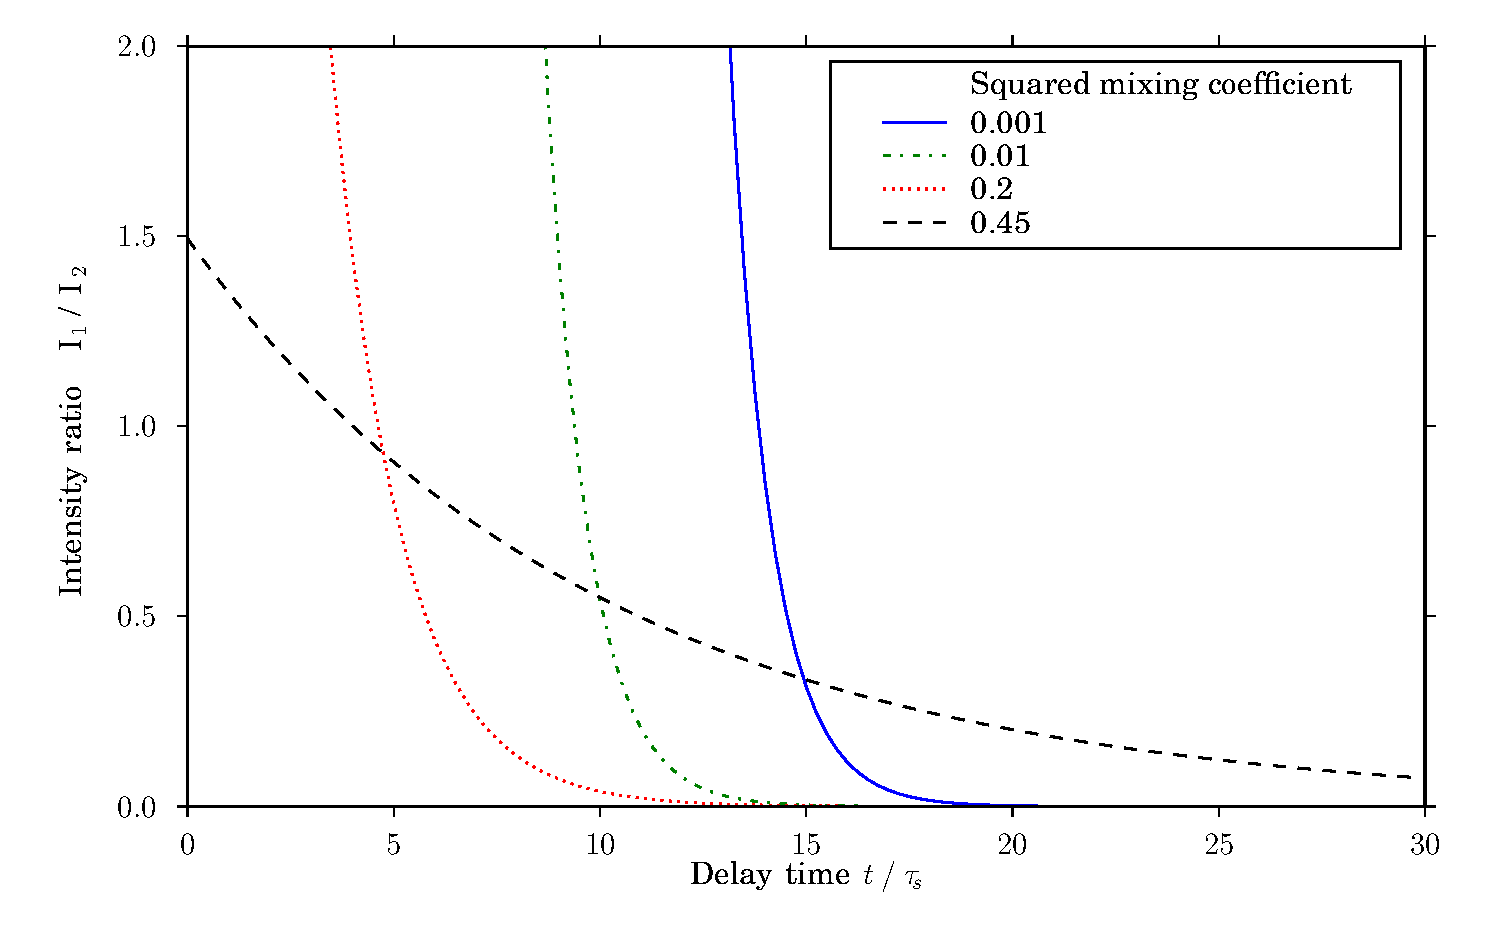
\includegraphics[width=6in]{ratio-development.pdf}
\end{figure}

The intensity-weighted center of gravity of the model system may be
written as a sum of two terms,
\begin{equation}
  E_{\text{ave}}(t) = E_1 \times I_1(t) \; + \; E_2 \times I_2(t),
\end{equation}
where $E_1$ and $E_2$ are the energies of $\ket{1}$ and $\ket{2}$,
respectively.  The intensity-weighted center of gravity is plotted as
a function of time delay in Figure \ref{fig:cog-devel}.  The main
features of the plot are similar to Figure \ref{fig:ratio-devel}.  At
small values of the mixing fraction, $0.001 \leq a^2 \leq 0.2$, the
center of gravity changes rapidly from $E_1$ to $E_2$ at a time delay
between $5\tau_s$ and $15\tau_s$.  When the mixing fraction is nearly
0.5, the initial center of gravity at $t=0$ is midway between $E_1$
and $E_2$, because $\ket{1}$ and $\ket{2}$ have similar intensities at
$t=0$.  In this case, the center of gravity changes slowly as a
function of time.  The quantity still approaches $E_2$ in the limit of
long time delay, because the lifetime of $\ket{2}$ is always longer
than that of $\ket{1}$.  The total magnitude of change in center of
gravity is decreased, due to the greater relative intensity of
$\ket{2}$ at $t=0$.

\begin{figure}
  \caption{Time development of the center of gravity for a model
    system containing two basis states.}
  \label{fig:cog-devel}
  \centering
  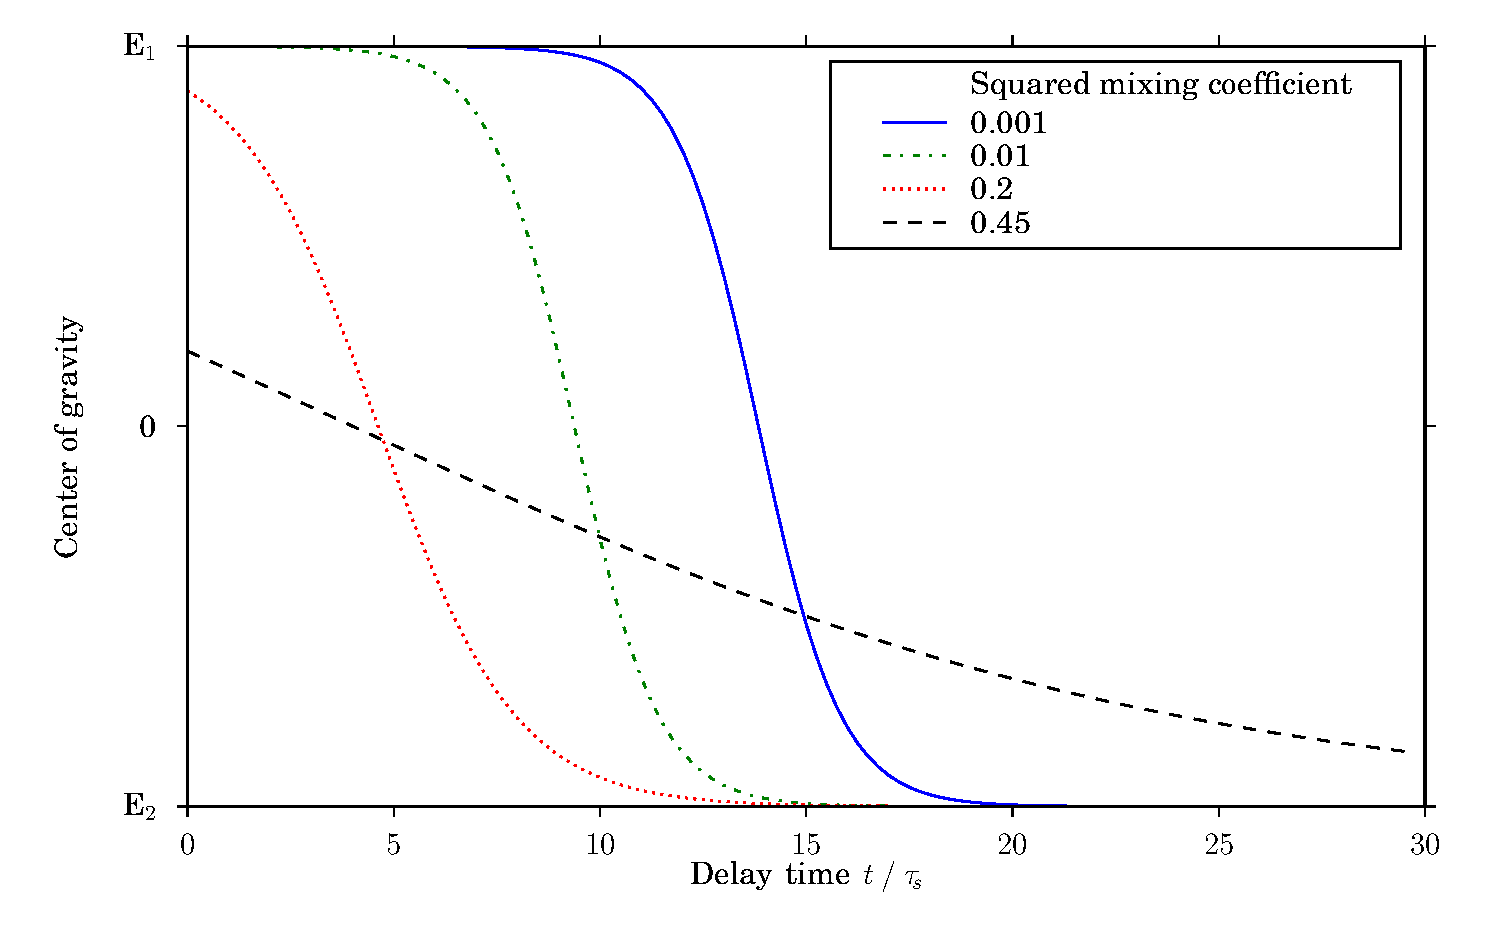
\includegraphics[width=6in]{cog-development.pdf}
\end{figure}

A characteristic feature in the plot center of gravity vs. time is the
presence and location of a rapid (within several $\tau_s$) shift in
center of gravity from $E_1$ to $E_2$.  If a rapid shift is observed,
its location may be used to infer the mixing fraction, $a^2$.  The
location of the shift is determined by the point of inflection for the
center of gravity function, where $I_1=I_2$.  The dependence of mixing
fraction on the location of a center of gravity shift is plotted in
Figure \ref{fig:cog-inflection-point}.  Rapid center of gravity shifts
located between $t=5.5\tau_s$ and $t=14\tau_s$ are the result of mixing
fractions between 0.1 and 0.001, respectively.

\begin{figure}
  \caption{The location of a rapid shift in center of gravity (taking
    place within several $\tau_s$) may be used to infer the $S_1 \sim
    T_3$ mixing fraction.  The location of the shift is given by the
    value of delay time where the relative intensities of the nominal
    $S_1$ eigenstate and the nominal $T_{1,2}$ eigenstates are equal.
    The mixing fraction is plotted here as a function of the location
    of a rapid shift in center of gravity.}
  \label{fig:cog-inflection-point}

  \centering
  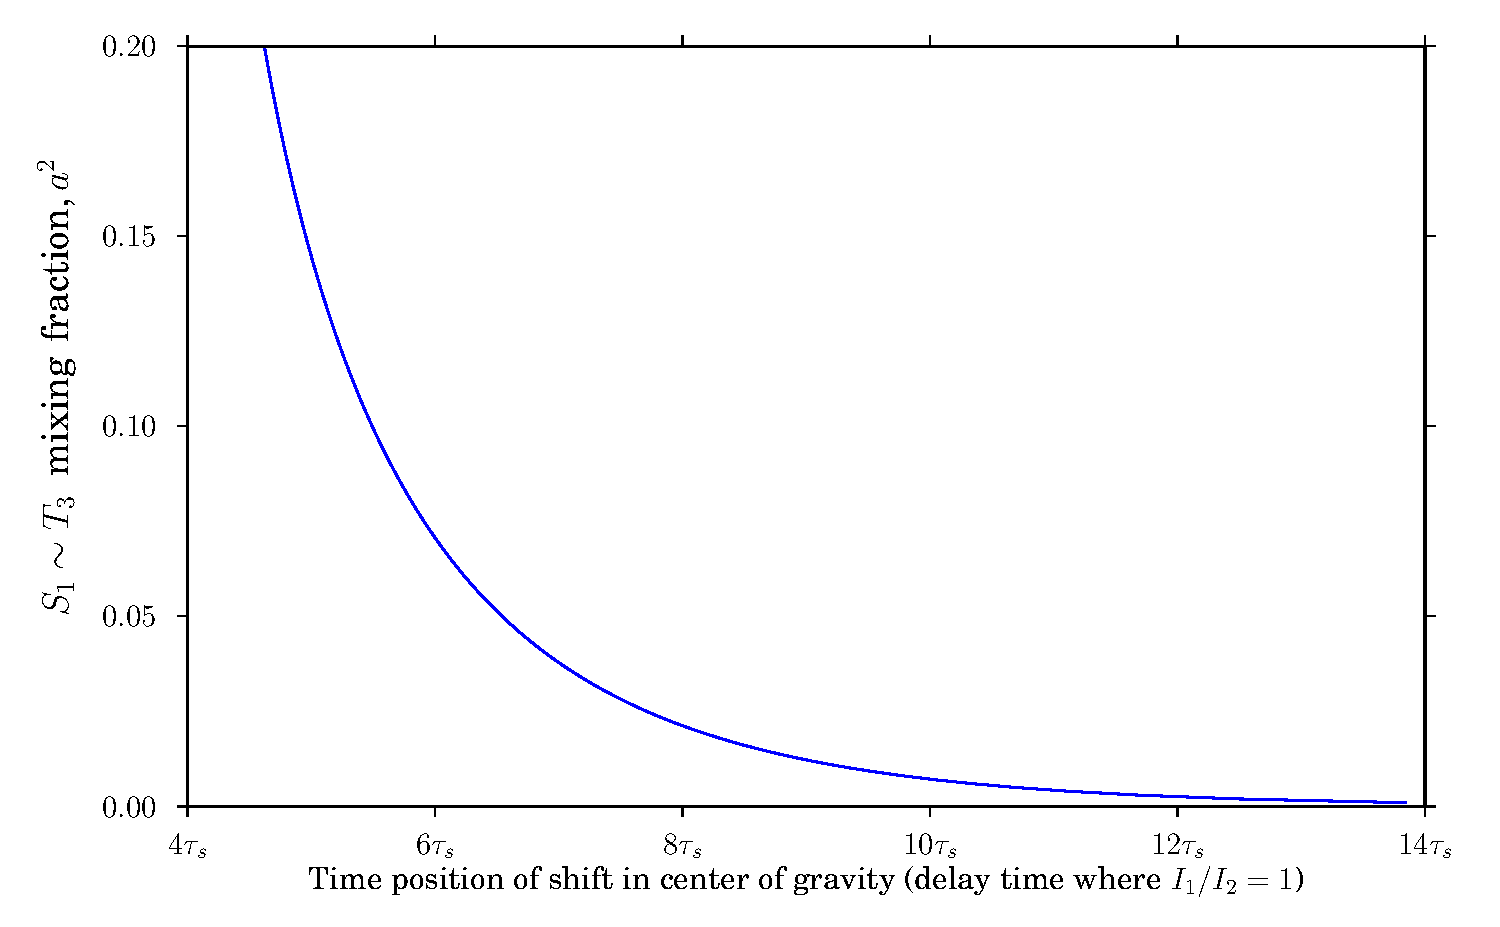
\includegraphics[width=6in]{cog-inflection-point.pdf}
\end{figure}

The presence of a rapid shift in center of gravity vs. time indicates
that the intensity ratio $I_1/I_2$ changes rapidly.  For this to
occur, the fluorescence decay rates of $\ket{1}$ and $\ket{2}$ must be
appreciably different.  For a system containing many $T_{1,2}$ levels,
the qualitative features of the center of gravity function will be
determined by the subset of nominal $T_{1,2}$ eigenstates with the
largest fractional $S_1$ character.  These states will have the
greatest intensities, and therefore the greatest impact on the
behavior of the center of gravity vs. time.  Therefore, the presence
of a rapid shift in center of gravity vs. time indicates that no
$T_{1,2}$ level is mixed to more than 20\% with the $S_1$ level.

We have examined the dependence of the intensity-weighted center of
gravity on time delay, in the LIF spectrum of an incoherent ensemble
of singlet$\sim$triplet mixed molecular eigenstates.  A model system
was constructed, containing one $S_1$ level and one $T_{1,2}$ level.
The initial $t=0$ position of the center of gravity for the model
system is influenced by the total $S_1 \sim T_{1,2}$ mixing fraction.
As the time delay is increased, the center of gravity shifts from its
initial $t=0$ position to a final position, which is determined solely
by the energy and fractional $S_1$ character of nominal $T_{1,2}$
eigenstates.  Small $S_1 \sim T_{1,2}$ mixing fractions lead to a
rapid, characteristic shift in the center of gravity with time delay.
Large mixing fractions lead to a gradual change in the center of
gravity with time delay.  In this case, the change in center of
gravity not only occurs more slowly, but the total magnitude of the
shift is decreased, due to the greater relative intensity of nominal
triplet states at $t=0$.

The behavior of the LIF center of gravity with time delay will be used
as a primary tool to examine the spectra of various vibrational
sublevels in acetylene \astate.  To analyze the local $S_1 \sim
T_{1,2}$ mixing around a single rotationally-resolved $S_1 \leftarrow
S_0$ trasition, relative intensities are compared over a very small
energy range, about 1 \rcm.  This has the effect of minimizing
relative intensity errors, which arise in LIF experiments mostly from
slowly drifting laser power and baseline effects.  Unlike measurements
of fluorescence lifetime, the center of gravity metric is not biased
by molecules leaving the LIF detection area.  Since the center of
gravity is determined by the relative fluorescence intensities among
molecules which remain within the field-of-view of the LIF detection
optics, the metric is unaltered as molecules exit the LIF detection
region, although the total signal is decreased.


























\section{Experiment}

In the SEELEM experiment, a molecular beam of acetylene is excited by
a $\sim$5 ns FWHM pulsed tunable laser into spin-rotation-vibration
eigenstates of metastable electronic states via weak, nominally
forbidden transitions. After excitation, the long-lived species must
travel 35 cm before colliding with an Au metal detector surface, where
an electron is ejected in a de-excitation process. Two criteria must
be met for electron ejection by a metastable species. First, the
vertical electronic energy of the metastable approaching the surface
must exceed the work function of the metal ($\Phi_{\text{Au}}$ = 5.1
eV). Second, the radiative lifetime of the detected metastable
eigenstate ($\tau_\text{rad}$) must exceed the flight time from the
point of laser excitation to the SEELEM surface ($\Delta$t=300
$\mu$s).

A sample of acetylene (BOC gases) at a backing pressure of one
atmosphere was pulsed through a 0.5 mm diameter nozzle (Jordan Valve)
operating at 10 Hz into a diffusion pumped vacuum chamber at
$\sim$5\e{-5} torr.  An Nd:YAG pumped (Spectra Physics GCR-270),
frequency-doubled dye laser (Lambda Physik FL3002, 220 nm) excited the
acetylene molecules in the pulsed jet expansion 2 cm downstream from
the nozzle orifice.  \TODO{Include laser details here.}

UV-LIF was detected perpendicular to the plane defined by the
intersection of the pulsed molecular and laser beams using f/1.2
collection optics, a fluorescence filter (UG-11) to reduce scattered
laser light, and a PMT (Hamamatsu model R375).  The time-varying
UV-LIF signal was averaged on a digital oscilloscope (LeCroy \TODO{get
  model}) at each laser frequency.  The resulting oscilloscope trace,
containing 500 evenly spaced voltage levels over a 5 \microsec\
timespan ($dt$ = 10 ns), was transferred to a PC for analysis.

Simultaneous SEELEM detection was performed in a separate,
differentially pumped vacuum chamber.  Following laser excitation,
molecules in the pulsed expansion passed through a conical skimmer
(3mm diameter), forming a collimated molecular beam in the SEELEM
detection chamber.  The detector chamber was diffusion pumped (Varian
600) to maintain a pressure of $\sim$4\e{-7} torr during operation.
The SEELEM detector surface, a 2.5 cm diameter region of heated
(300\degrees\ C) Au foil, was located 35 cm downstream from the point
of laser excitation.  The SEELEM detector was identical to that used
in the previously described apparatus with Au foil ($\Phi_{\text{Au}}$
= 5.1 eV) as the detector surface.

Electron signals from the SEELEM detector were collected using pulse
counting techniques.  Electrons ejected from the metal surface were
detected by a nearby electron multiplier (ETP, SGE Instruments, Model
14831H).  The collection plate of the multiplier was biased at +100V
to attract electrons.  The electron multiplier signal was sent to a
discriminator (EG\&G/Ortec Model 9301), and then to a PC-operated
multichannel scalar (Oxford Tennelec Nucleus Inc. MCS-II v2.091),
where the total number of electrons was summed.  The typical signal
level for SEELEM detection of acetylene was 2-20 counts per laser
pulse.

Both SEELEM and LIF signals were averaged over 100 laser shots at each
laser frequency.  The frequency increment was typically $\sim$0.015
\rcm\ in the doubled output, although several detailed spectra were
recorded with a 4$\times$ smaller frequency step size.





























\section{SEELEM/LIF spectroscopy of four $S_1$ vibrational levels
  above the minimum of the $S_1 \sim T_3$ seam of intersection}


The choice of $S_1$ vibrational levels in this study was guided by two
considerations: the energetic accessibility of $T_3$ vibrational
levels \cite{cui97, thom07} and absence of predissociation effects.
The minimum of the $S_1 \sim T_3$ electronic seam of intersection,
located near $3^3$ \Ka{1}, $T_0 \simeq 45300$ \rcm, provides a lower
energy bound for the Franck-Condon accessibility of $T_3$ vibrational
levels from the $S_1$ electronic surface \cite{cui97}.  Above this
energy, any $S_1$ level may, in principle, have a large vibrational
overlap with one or more $T_3$ levels.  The first dissociation
barrier, located near $3^4$ \Ka{1}, $T_0 \simeq 46300$ \rcm, provides
an upper energy bound for this study \cite{mordaunt98}.  Below this
barrier, predissociation pathways are not energetically accessible,
and do not complicate the study of $S_1 \sim T_3$ interactions.

We consider four $S_1$ sublevels in this energy region, observed in
the $\tilde{A}^1A_u \leftarrow \tilde{X} ^1\Sigma_g^+$ spectrum of
acetylene.  The sublevels are listed with their total (rotationless)
vibronic energy, $T_0$, in Table \ref{table:termvals}.  Included in
the table is an order-of-magnitude estimate of the SEELEM:LIF
intensity ratio observed in the spectrum.  To determine this quantity,
the relative LIF intensties of $2^23^1$ \Ka{1}, $3^24^2$ \Ka{1}, and
$2^13^2$ \Ka{1} were estimated from a low resolution jet spectrum
reported by Merer and coworkers \cite{merer03}.  The LIF intensity of
the $3^3$ \Ka{2} subband was compared to that of $3^3$ \Ka{1} in our
own experiments.  The absolute SEELEM intensity was then divided by
the estimated LIF intensity, and normalized to the largest SEELEM:LIF
ratio.


%%%%%%%%%%%%%%%%%%%%%%%%%%%%%%%%%%%%%%%%%%%%%%%%%%%%%%
%%
%% INSERT LEVEL TABLE HERE
%%
%%%%%%%%%%%%%%%%%%%%%%%%%%%%%%%%%%%%%%%%%%%%%%%%%%%%%%

\begin{table}
  \caption{The four acetylene $S_1$ vibrational levels considered in
    this study, listed here, have total vibronic energies in the
    critical region above the minimum of the $S_1 \sim T_3$ electronic
    seam of intersection ($\simeq 45300$ \rcm) and below the first
    dissociation barrier ($\simeq 46300$ \rcm).  An order-of-magnitude
    estimate of the observed SEELEM:LIF intensity ratio is included.}
  \label{table:termvals}

  \centering
  \begin{tabular}{rlrr}
    \\
    Subband & & $T_0$ (\rcm ) & SEELEM:LIF\\
    \midrule
    $2^23^1$ \Ka{1} & $\leftarrow$ $0_0$ & 46009 & $10^{-2}$ \\
    $3^24^2$ \Ka{1} & $\leftarrow$ $0_0$ & 45812 & $10^{-1}$ \\
    $2^13^2$ \Ka{1} & $\leftarrow$ $0_0$ & 45677 & $10^{-1}$ \\
      $3^3$ \Ka{2} & $\leftarrow$ $4_1$ & 45352 & 1 \\
  \end{tabular}
\end{table}

%%%%%%%%%%%%%%%%%%%%%%%%%%%%%%%%%%%%%%%%%%%%%%%%%%%%%%
%%
%% END OF LEVEL TABLE
%%
%%%%%%%%%%%%%%%%%%%%%%%%%%%%%%%%%%%%%%%%%%%%%%%%%%%%%%



We observe that the highest energy state in our study has the lowest
SEELEM:LIF intensity ratio.  Rather than total energy, the SEELEM:LIF
intensity ratio is determined by the number of quanta in mode 3.  This
observation is in agreement with previous estimations of SEELEM:LIF
intensity ratios in acetylene \astate\ \cite{humphrey97}.
Measurements of the Zeeman anticrossing density show the same
exponential dependence on the number of quanta in $\nu_3$
\cite{dupre91}.  Because the intensity ratio is determined by
vibrational basis state character and not by total energy, it must be
an effect of the vibrational overlap factors contained in spin-orbit
matrix elements, rather than an effect of the slowly increasing
density of $T_{1,2}$ states \cite{dupre91, dupre95b}.

We observe no systematic splittings at adjacent rotational levels in
any of the spectra, which would indicate the presence of a
near-degenerate $T_3$ doorway vibrational level, as in $3^3$ \Ka{1}
\cite{mishra04}.  Evidence of energetically distant $T_3$ doorway
levels is found, however, in both the SEELEM and LIF spectra of these
sublevels.  To characterize the spectral signatures of energetically
distant doorway levels, we discuss the SEELEM/LIF spectrum of each
sublevel individually.


\subsection{The $3^24^2$ \Ka{1} sublevel: evidence for an
  energetically distant $T_3$ doorway level plus a localized $T_3$
  level crossing}

% Spectrum: Dec05n 2006, p.86 of 9/2006--1/2007 notebook.

%%%%%%%%%%%%%%%%%%%%%%%%%%%%%%%%%%%%%%%%%%%%%%%%%%%%%%
%%
%% INSERT 3^2 4^2 FIGURES HERE
%%
%%%%%%%%%%%%%%%%%%%%%%%%%%%%%%%%%%%%%%%%%%%%%%%%%%%%%%


\begin{figure}
  \caption{Simultaneously recorded SEELEM (upper trace) and LIF (lower
    trace) spectra of the $3^24^2$ \Ka{1} sublevel of the \astate\
    state of \ce{C2H2}.  The LIF spectrum is integrated in two time
    regions: an early time window ($0.5\tau_s-2\tau_s$, solid trace)
    and a delayed time window ($10\tau_s-18\tau_s$, dashed trace).
    The peak positions are blueshifted in the delayed fluorescence
    spectrum for all transitions, with the exception of Q(2).
    Interactions with a remote perturber level of slightly lower
    energy are apparent in the delayed fluorescence spectrum of the
    Q(2) and R(1) transitions.}
  \label{fig:spectrum-32b2}
  \centering
  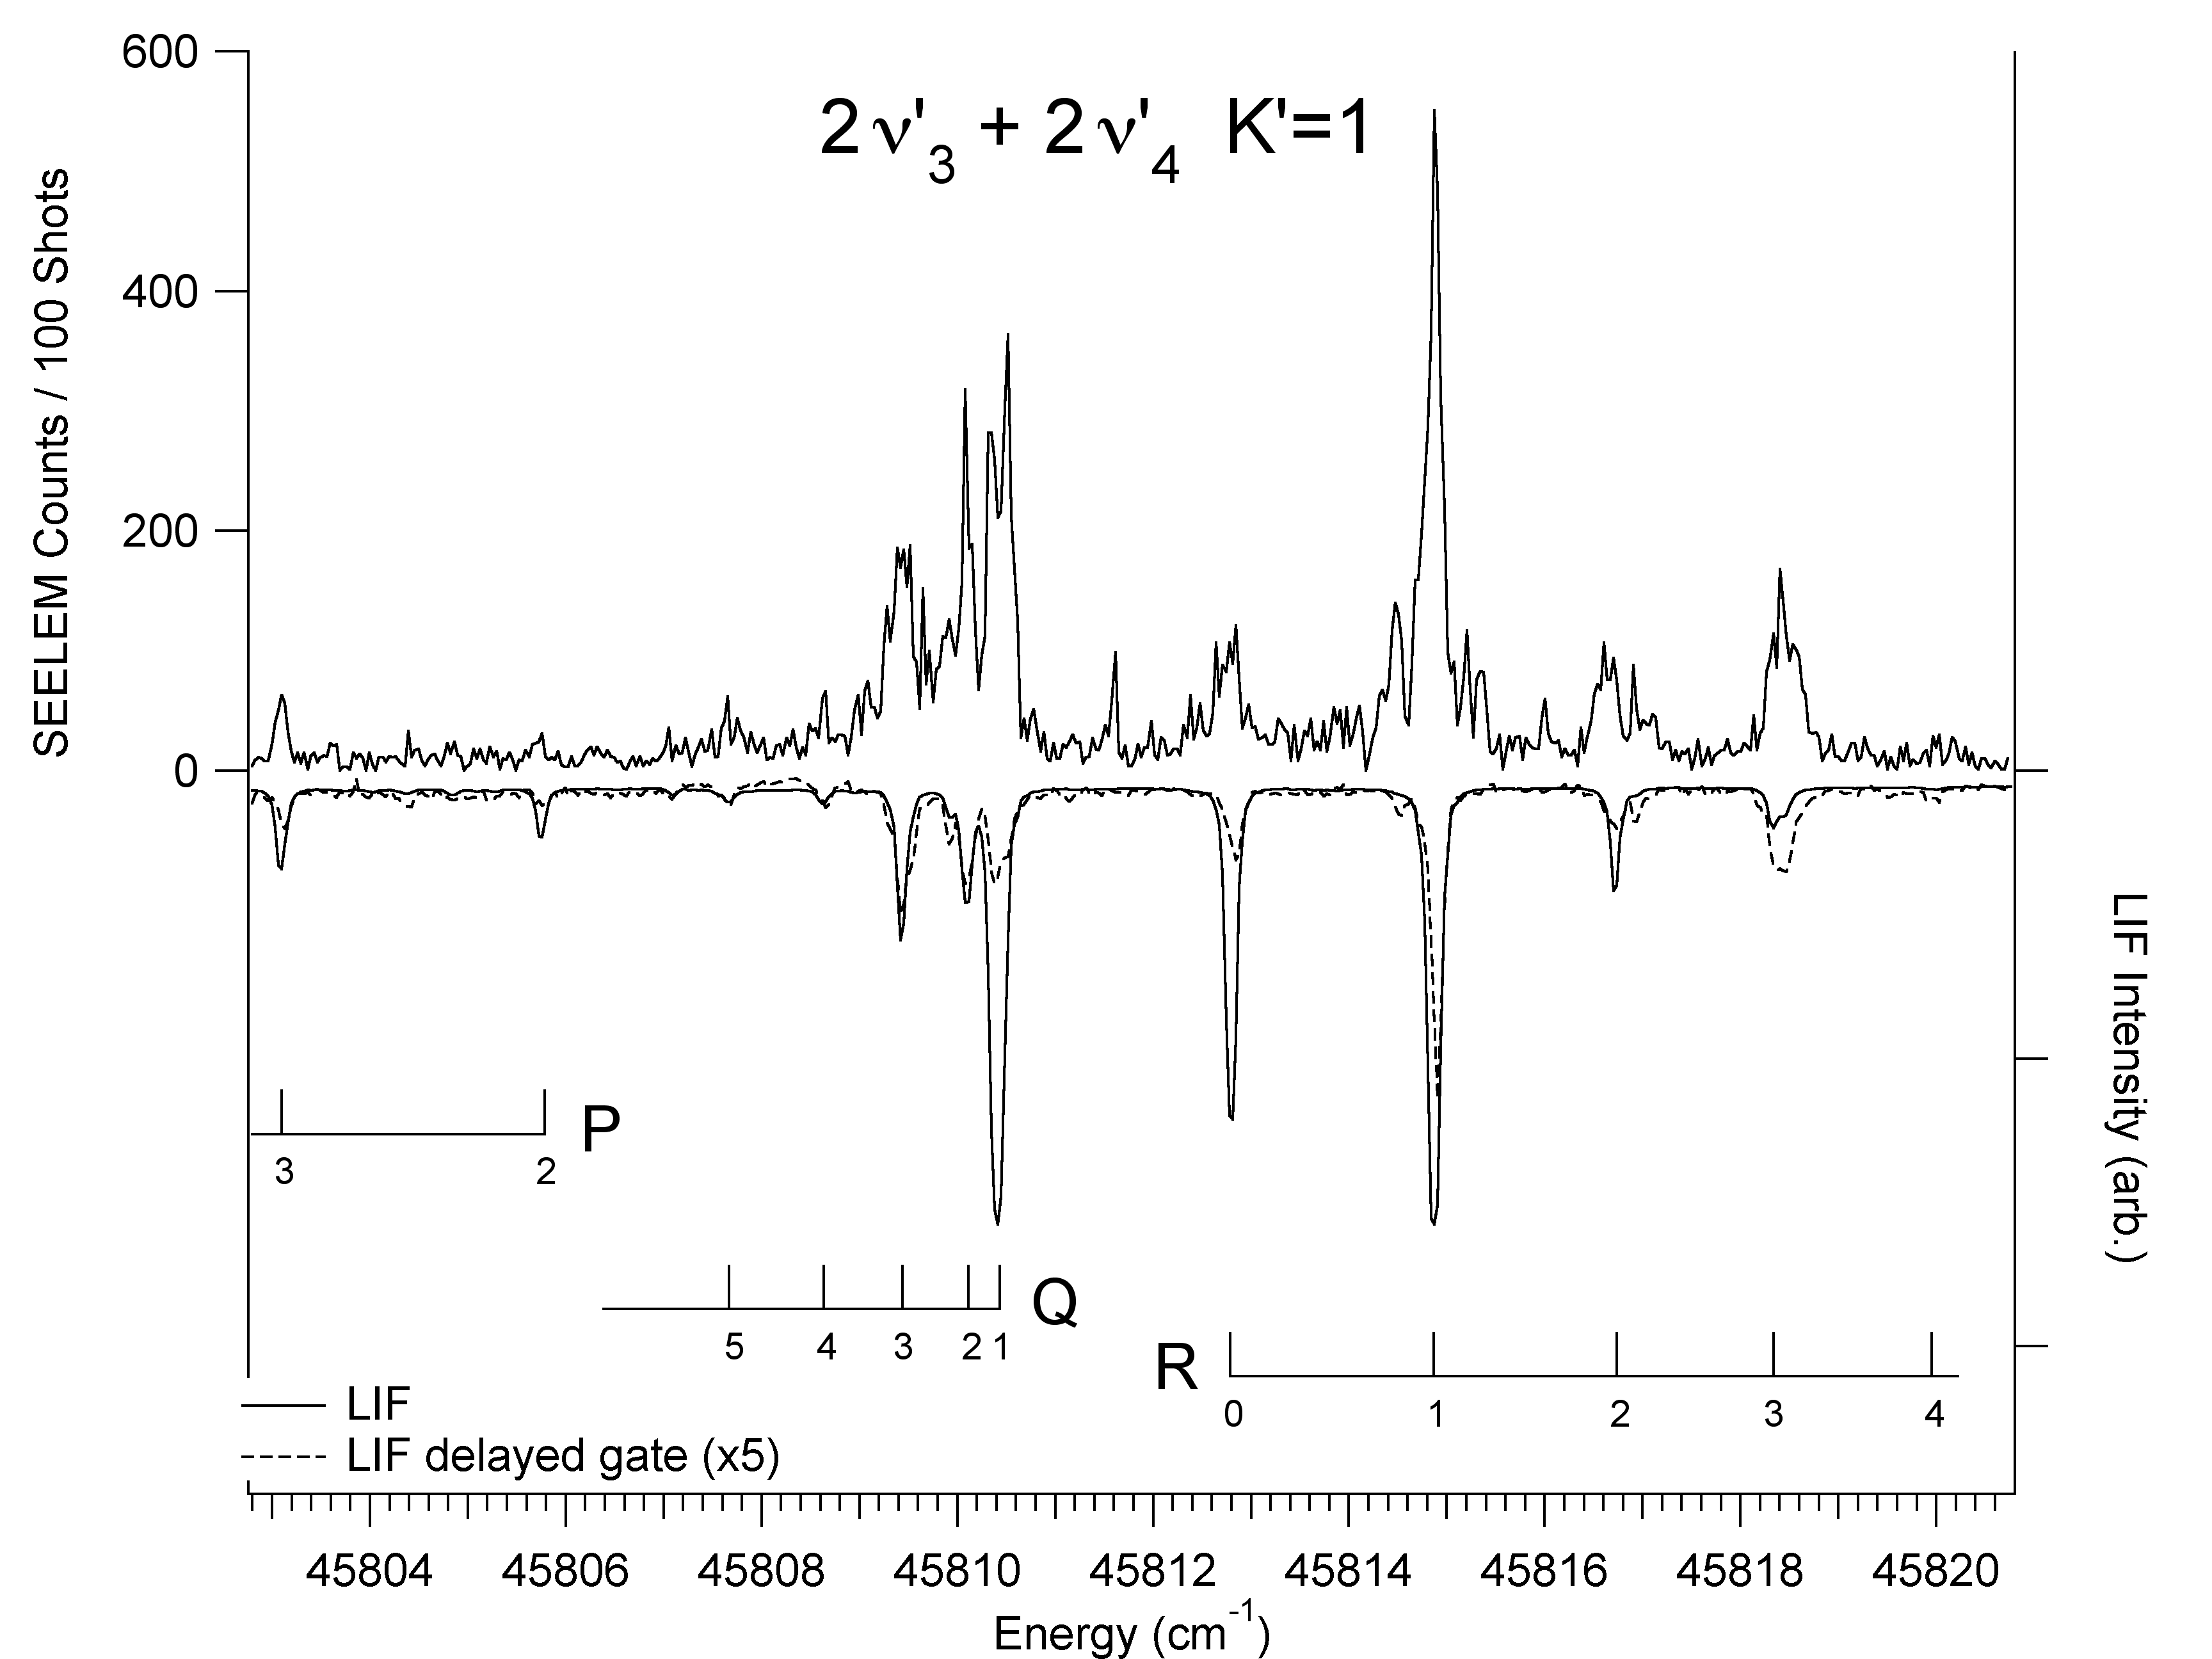
\includegraphics[width=7in,angle=90]{acetylene-32b2-p3r4.png}
\end{figure}

\begin{figure}
  \caption{Dependence of the intensity-weighted center of gravity on
    delay for a series of individually resolved transitions, Q(1$-$3)
    (top), and R(0$-$3) (bottom), in the LIF spectrum of $3^24^2$
    \Ka{1}.  Local perturbations in the Q(2) and R(1) transitions
    cause the center of gravity to deviate from those of the other
    transitions as the delay time is increased.}
  \label{fig:32b2-cog-delay}
  \centering
  \vspace{5mm}
  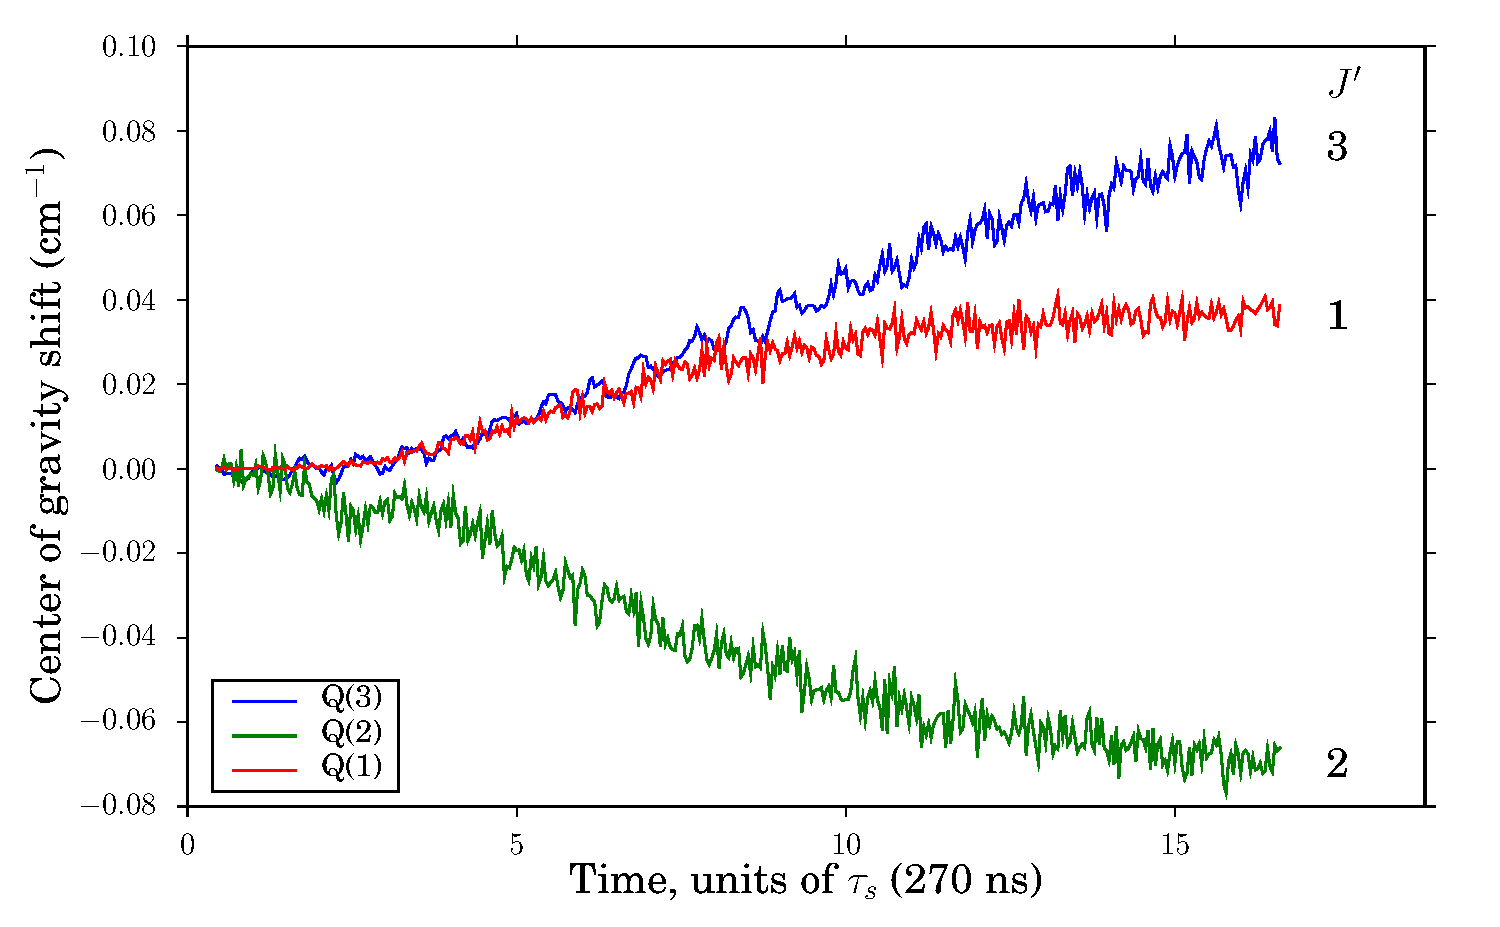
\includegraphics[width=6in]{32b2-q123-cog-delay.pdf}
  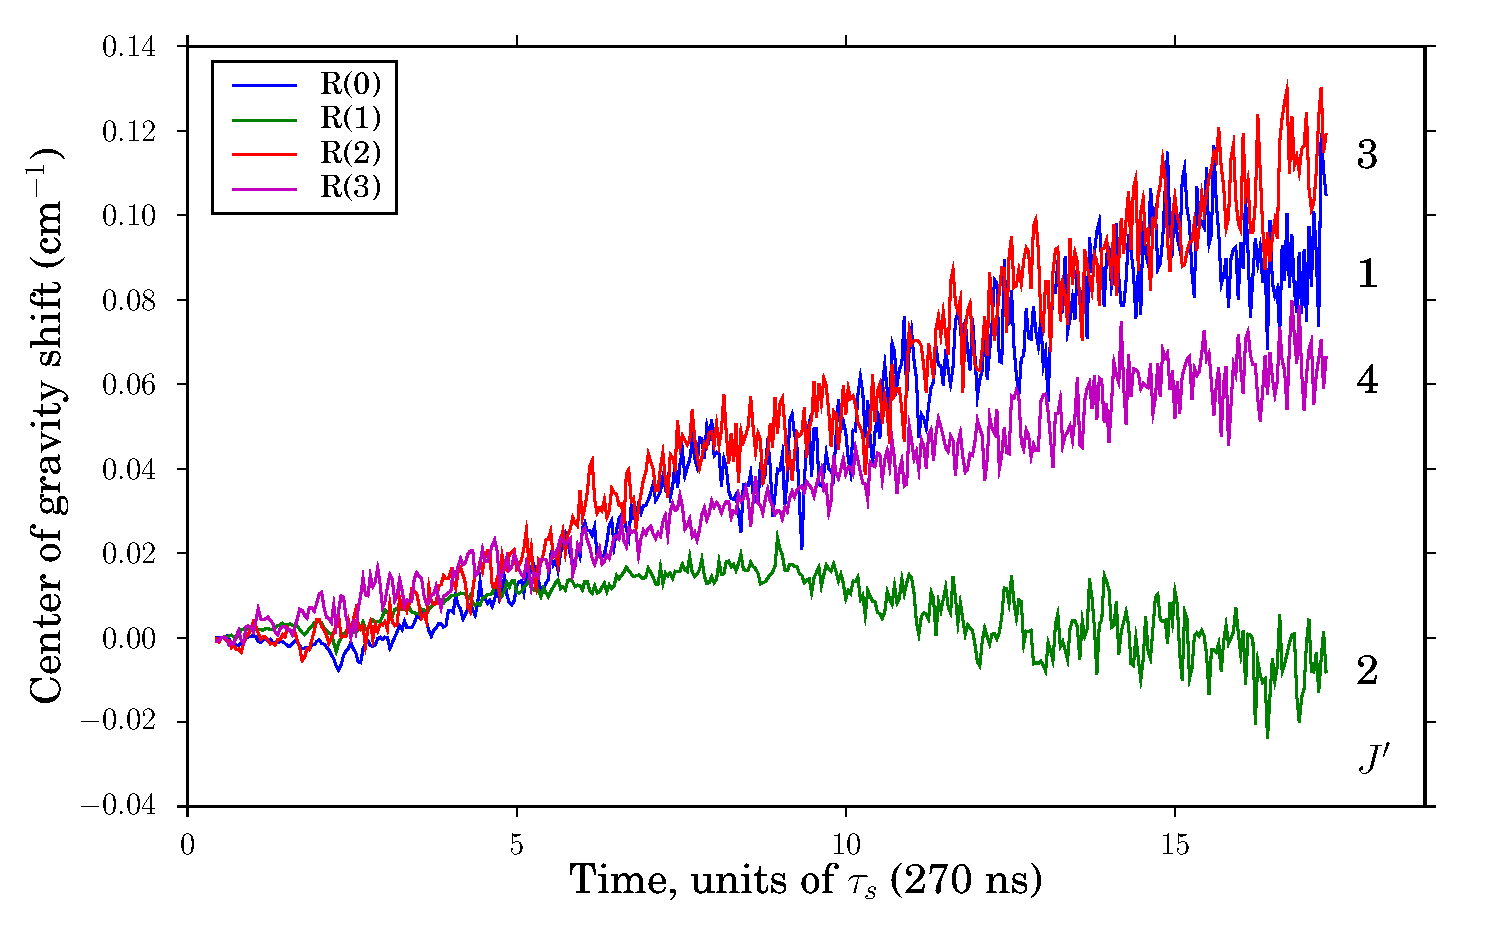
\includegraphics[width=6in]{32b2-r0123-cog-delay.pdf}
\end{figure}


%%%%%%%%%%%%%%%%%%%%%%%%%%%%%%%%%%%%%%%%%%%%%%%%%%%%%%
%%
%% END OF 3^2 4^2 FIGURES
%%
%%%%%%%%%%%%%%%%%%%%%%%%%%%%%%%%%%%%%%%%%%%%%%%%%%%%%%

The $3^24^2$ level is the upper member of the $3^2B^2$ polyad of the
acetylene \astate state, where the vibration $\nu_B$ represents either
$\nu_4$ or $\nu_6$.  The $\nu_4$ and $\nu_6$ vibrations are strongly
mixed by a-type Coriols and Darling-Dennison anharmonic resonances
\cite{merer08}.  As a result, the nominal $3^24^2$ level is expected
to contain essentially a 50:50 mixture of mode 4 and mode 6 basis
character \cite{merer08, virgo07}.

The simultaneously recorded SEELEM/LIF spectrum of the $3^24^2$ \Ka{1}
$\leftarrow$ $0_0$ subband of the \AtoX\ electronic spectrum is shown
in Figure \ref{fig:spectrum-32b2}. To highlight the dependence of the
LIF spectrum on delay time, two integration regions are used.  An
early LIF fluorescence spectrum is generated by gating the
fluorescence signal between $0.5\tau_s$ and $2\tau_s$.  A second,
delayed LIF spectrum is generated from integration in the time window
$10\tau_s-18\tau_s$.  The peak poisitions of several transitions are
clearly blueshifted in the delayed LIF spectrum relative to the early
LIF.  Peak offsets in the R(0), R(1), and R(4) transitions are
approximately 0.08 \rcm.

To more closely examine the dependence of the LIF spectrum on time
delay, the intensity-weighted center of gravity (Formula (from last
section)) is plotted for each transition as a function of delay time.
The plot for Q-branch transitions was generated from another dataset,
not shown here, sampled at approximately $4 \times$ more closely
spaced energy intervals, resulting in increased signal to noise.  With
the exception of the R(1) and Q(2) transitions, the center of gravity
increases by 0.04-0.12 \rcm\ over the delay range
$0.5\tau_s-18\tau_s$.  Such a consistent increase in center of gravity
with delay time indicates the presence of a non-local $T_3$ doorway
level that lies higher in energy, according to Formula (from
preceeding section).

% The interaction is observed in both parities of the singlet at
% $J'=1$ and $3$.  A doorway level with $K_T=0$ would The doorway
% level cannot be assigned as $K_T=0$.  \emph{e}/\emph{f} symmetry
% selection rules the interaction is present in both parities of the
% singlet, .  Two possibilities remain for $K_T$

A line splitting is present in the LIF spectrum of two transitions,
Q(2) and R(1).  The relative intensities of the extra levels in the
delayed fluorescence is stronger than that of the main component of
the transition, indicating that they arise from levels with longer
zero-order fluorescence lifetimes than that of the singlet.  The extra
line in R(1) is observable only in the delayed LIF spectrum, where its
relative intensity increase causes it to emerge from under the red
wing of the main line.  The extra line in the R(1) transition, having
upper state quantum number $J'=2$, is located at an energy of -0.33
\rcm\ below the main component at 45814.87 \rcm.  The perturber of
Q(2), also having $J'=2$, is located at an energy of -0.17 \rcm\
relative to the peak of the strong, nominally singlet LIF transition
at 45810.08 \rcm.

The presence of two local perturbations at the same $J'$, arising from
levels with a long zero-order lifetime, and not appearing in
transitions with adjacent values of $J'$, can be explained by the
presence of a level crossing involving the $F_1$ or $F_3$ component of
a $T_3$ level having a small spin-orbit matrix element with the $S_1$
level.  According to Formula (from last section), the relative energy
of a $T_3$ level in this case is $\pm 2B \simeq \pm 2$ \rcm\ at $J'=1$
and $3$.  At $J'=2$, the singlet and its triplet perturber are not
50:50 mixed, thus the matrix element must be appreciably smaller than
half the energy separation.  This places an upper bound on the matrix
elements of about $0.01$ \rcm.  At $J'=1$ or $3$, the increase in
energy denominator from 0.2 \rcm\ to 2 \rcm\ would make the intensity
of the perturber $100$ times weaker than for $J'=2$, precluding its
observation in LIF.

A lone SEELEM peak is observed in the band gap at 45811.6 \rcm,
approximately 2 \rcm\ above the Q(3) transition at 45809.5 \rcm.  It
is possible that this peak arises from the same weakly perturbing
$T_3$ vibrational level.  Unfortunately, this energy region is
overlapped in the spectrum by another R-branch transition, so it is
impossible to look for the perturber in the other parity in this
spectrum.  However, if we assign the transition in the band gap as
$J'=3$, it must also be assigned as the $F_3$ component of the triplet
level, $N_T=J'+1=4$, in order to be located at $+2$ \rcm\ instead of
$-2$ \rcm.  As a consequence, the triplet level must have a
rotationless vibronic energy of $45811 - 6B \simeq 45804$ \rcm.

We have examined a singlet sublevel, $3^24^2$ \Ka{1}, which shows
evidence of interaction with an energetically distant $T_3$ doorway
level at higher energy.  An extra line with a small matrix element was
observed at $J'=2$ in both parity components of the singlet level, and
was assigned as a level of $T_3$ baased on its zero-order lifetime.
An assignment of $\Delta N=+1$ was suggested for the perturbing level
based on the observation of a weak transition in the SEELEM spectrum,
which was assigned as $J'=3$, $N_T=4$ due to its energy of $+2$ \rcm\
relative to the singlet Q(3) transition.  The assignment of $N_T$
determines that the rotationless energy of the perturbing triplet
level is $-6$ \rcm\ relative to the singlet. 

If the assignment of $N_T$ is not made from the observed SEELEM
transition at 45811.6 \rcm, the extra line in Q(3) may belong to
either the $F_1$ ($\Delta N = -1$) or $F_3$ ($\Delta N = +1$)
component of the perturbing $T_3$ level.  In this circumstance, the
additional possibility for assignment of $N_T$ means that the
perturbing $T_3$ level may also be located at an energy of $+4$ \rcm\
relative to the singlet.

Local, weak perturbations by $T_3$ levels are common in the spectrum
of \astate\ acetylene, as we will see in the following examples.  In
cases where $N_T$ or $K_T$ of the perturber can be assigned, the
relative energies of weak, locally perturbing vibrational levels can
be determined exactly.  In cases where $N_T$ or $K_T$ can be assigned
for energetically distant $T_3$ doorway levels (levels with large
matrix elements), the relative rotationless energy is determined to be
either positive or negative.  This can then be checked against the
dependence of the intensity-weighted LIF center of gravity on time
delay.

\subsection{The $2^13^2$ \Ka{1} sublevel: assignment of $K_a$ for an
  energetically distant $T_3$ doorway level}

% Spectrum: Jan 16A+B, p.124--127 of 9/2006--1/2007 notebook, also
% assignments on p.2 of 1/2007--3/2007 notebook.

%%%%%%%%%%%%%%%%%%%%%%%%%%%%%%%%%%%%%%%%%%%%%%%%%%%%%%
%%
%% INSERT 2^1 3^2 FIGURES HERE
%%
%%%%%%%%%%%%%%%%%%%%%%%%%%%%%%%%%%%%%%%%%%%%%%%%%%%%%%

\begin{figure}
  \caption{Simultaneously recorded SEELEM (upper trace) and LIF (lower
    trace) spectra of the $2^13^2$ \Ka{1} sublevel of the \astate\
    state of \ce{C2H2}.  The LIF spectrum is integrated in two time
    regions: an early time window ($0.5\tau_s-2\tau_s$, solid trace)
    and a delayed time window ($10\tau_s-18\tau_s$, dashed trace).
    The Q(1) and Q(2) transitions are redshifted in the delayed
    fluorescence spectrum, in contrast to the Q(3,4,5,6) transitions.
    The P(2) and Q(1) transitions, having the same $J'$ but opposite
    parity, show similar redshifts in the delayed fluorescence
    spectrum.}
  \label{fig:spectrum-2132}
  \centering
  \vspace{1cm}
  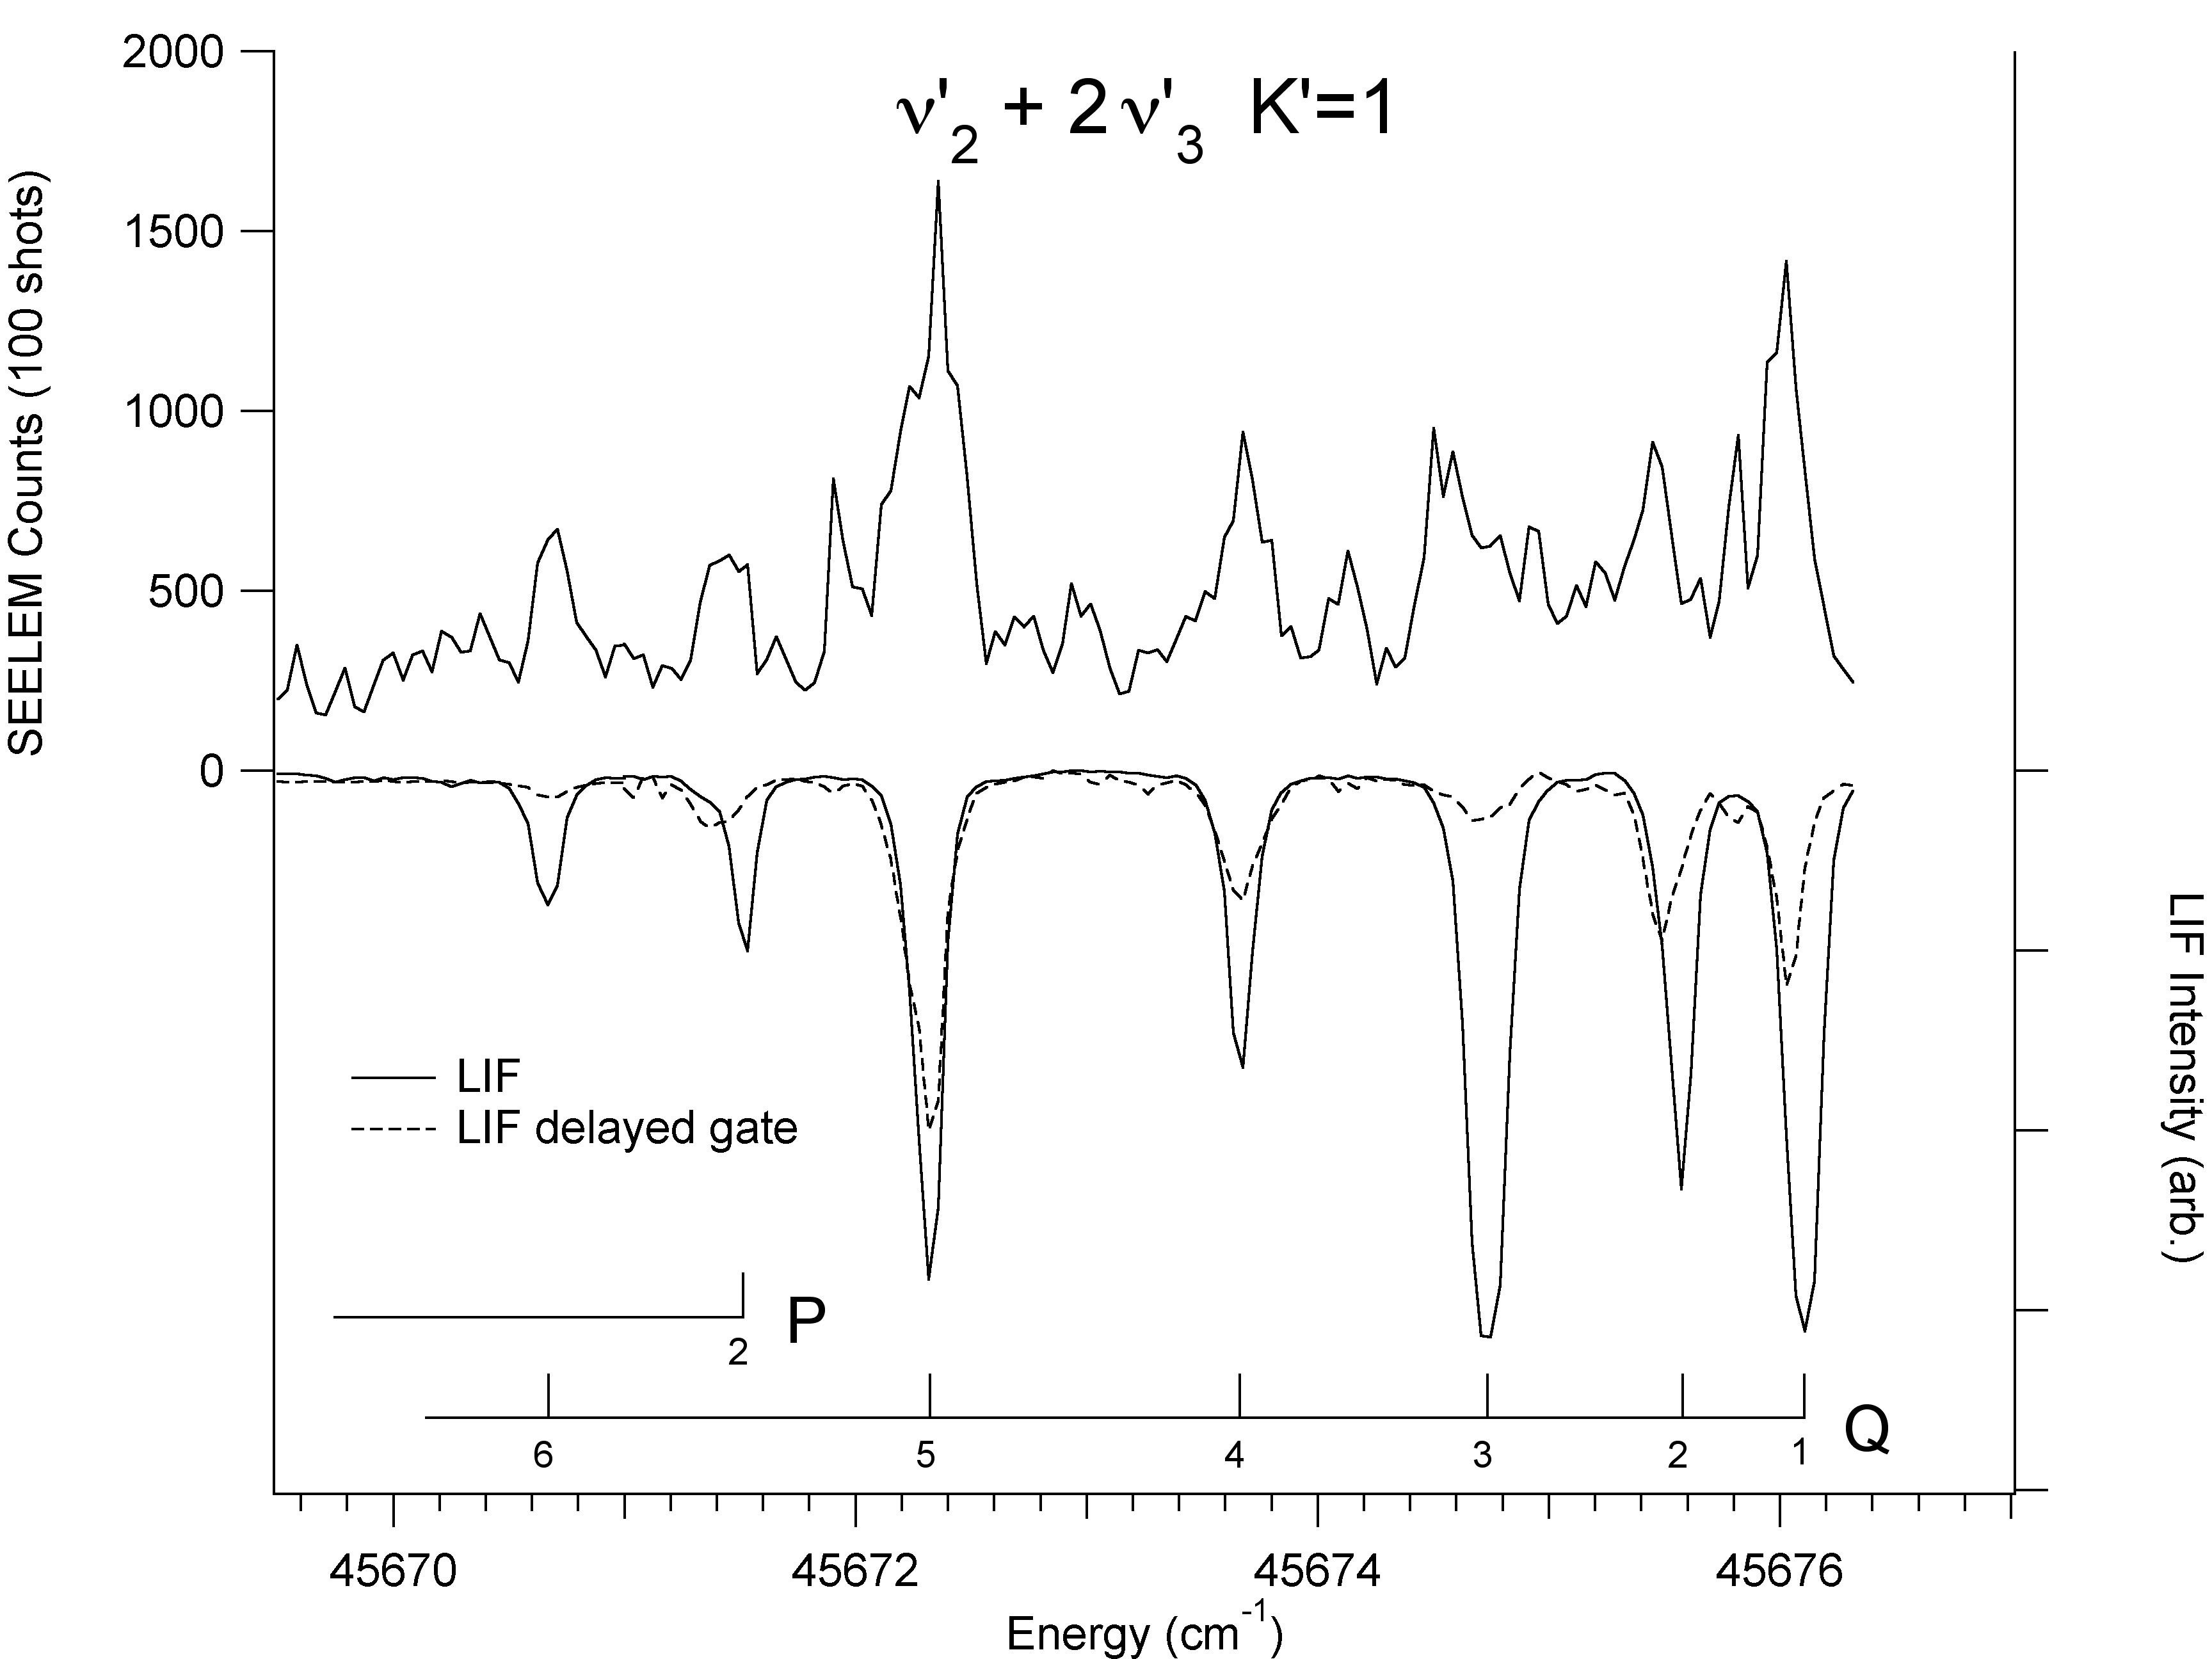
\includegraphics[width=7in,angle=90]{acetylene-2132-q6q1.png}
\end{figure}

\begin{figure}
  \caption{Dependence of the intensity-weighted center of gravity on
    delay for a series of individually resolved rotational
    transitions, Q(1$-$5), in the LIF spectrum of $2^13^2$ \Ka{1}.
    The center of gravity of the Q(1) and Q(2) transitions is
    identical to the the peak positions in the SEELEM spectrum at
    delay $>$ $15\tau_s$.}
  \label{fig:2132-q123456-cog-delay}
  \centering
  \vspace{1cm}
  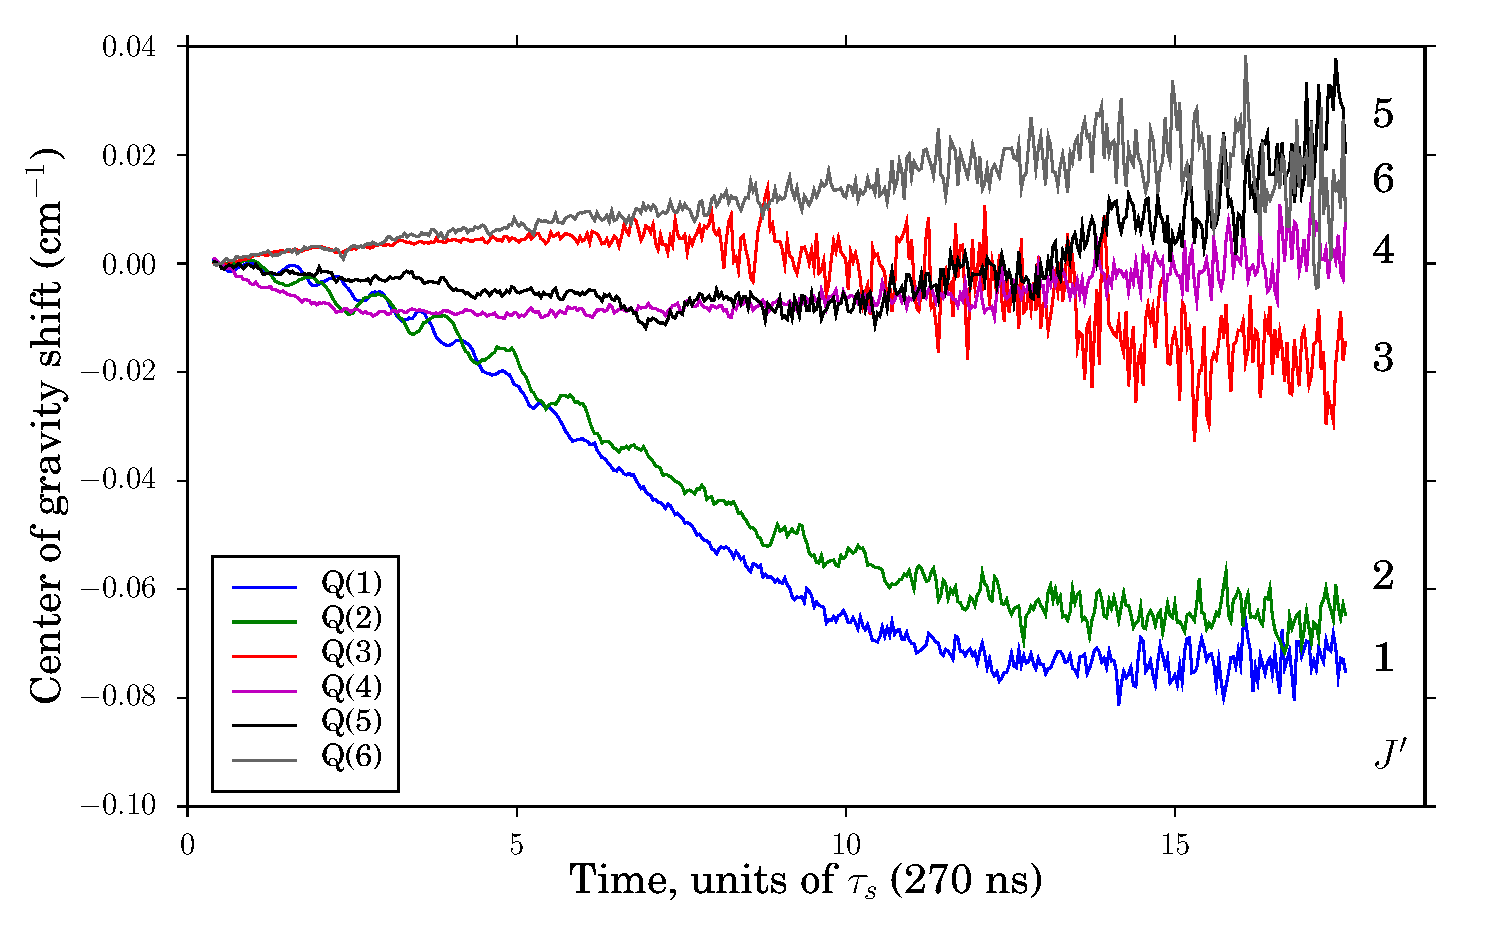
\includegraphics[width=6in]{2132-q123456-cog-delay.pdf}
\end{figure}

%%%%%%%%%%%%%%%%%%%%%%%%%%%%%%%%%%%%%%%%%%%%%%%%%%%%%%
%%
%% END OF 2^1 3^2 FIGURES
%%
%%%%%%%%%%%%%%%%%%%%%%%%%%%%%%%%%%%%%%%%%%%%%%%%%%%%%%

We turn next to an $S_1$ sublevel which also contains two quanta of
the $\nu_3$ vibration, $2^13^2$ \Ka{1}.  The overall SEELEM:LIF
intensity ratio observed in the spectrum of this sublevel is similar
to that of $3^24^2$ \Ka{1}, indicating a similar overall mixing angle
with $T_3$ doorway levels.

The SEELEM/LIF spectrum of the $2^13^2$ \Ka{1} $\leftarrow$ $0_0$
subband of the \AtoX\ transition is shown in Figure
\ref{fig:spectrum-2132}.  The LIF spectrum is integrated in early and
delayed time windows, using time limits of $0.5\tau_s-2\tau_s$ and
$10\tau_s-18\tau_s$.  The spectrum contains six Q-branch transitions
(upper states of \emph{f}-symmetry, $J'=1-6$) and one P-branch
transition (upper state of \emph{e}-symmetry, $J'=1$).  The delayed
LIF peak position is redshifted by -0.08 \rcm\ relative to the early
LIF peak position for two transitions terminating in \emph{f}-symmetry
states, Q(1) and Q(2).  The sole \emph{e}-symmetry state observed in
the spectrum, via the P(2) transition, is also redshifted in the
delayed fluorescence spectrum by -0.12 \rcm.  The remaining
transitions, Q(3,4,5,6), have the same peak position in the early and
delayed LIF spectra.

The dependence of the intensity-weighted center of gravity for all
transitions in the Q-branch is shown in Figure
\ref{fig:2132-q123456-cog-delay}.  The center of gravity for the Q(1)
and Q(2) transitions changes from the zero-delay position by
approximately -0.07 \rcm\ at a time delay of $15\tau_s$, in accord
with the observation of delay-dependent peak positions in the LIF
spectrum.  The center of gravity for the Q(3,4,5,6) transitions does
not shift by more than 0.02 \rcm\ from its initial position.

We came to the conclusion in the preceeding section that a consistent
shift in center of gravity with delay indicates the presence of an
energetically distant $T_3$ doorway level.  It is puzzling that, in
this case, such an interaction abruptly ceases at $J'=3$.  However,
this behavior can be explained by the presence of a \emph{second}
$T_3$ doorway level, located at higher energy than the singlet level.
An interaction with a second $T_3$ doorway level could cause the
delayed center of gravity to behave differently for the Q(3,4,5,6)
transitions, if the interaction were to \emph{begin} at $J'=3$.

The existence of such an interaction leads to an assignment of $K_T$
for the second doorway level.  The spin-orbit selection rule $\Delta K
= 0, \pm 1$ restricts possible assignments to $K_T=$0, 1, and 2.  A
level with $K_T=2$ has rotational levels that begin with $N_T=2$.  An
$S_1 \sim T_3$ interaction with the $F_1$ component of such a level
follows the selection rule $\Delta N = -1$, and would first turn on at
$J'=N_S \geq 3$, as observed in the spectrum.  All other combinations
of $\Delta K$ and $\Delta N$ lead to $S_1 \sim T_3$ interactions
starting at $J' \geq 1$ or $2$.  Thus, we can assign $K_T=2$ for the
second $T_3$ doorway level.

For the $F_1$ component of a triplet level, the energy of the triplet
relative to the singlet has a negative slope with respect to $J'$ (see
Figure \ref{rotational-energy-differences}).  At $J'=3$, where the
interaction with the second doorway level begins, the $F_1$ component
is $6B \simeq 6$ \rcm\ lower in energy than the $F_2$ component.  As
$J'$ increases, the relative energy of the $F_1$ component decreases
by $2B$ per $J'$.  Since the interaction must occur through an $F_1$
component in order to turn on at $J'=3$, and since the relative energy
of the $F_1$ component is appreciably lower than that of the other two
components, we must conclude from the assignment of $K_T$ that the
second $T_3$ doorway level is higher in energy than the singlet level.
% This is, in fact, what is deduced from in the dependence of
% intensity-weighted center of gravity on delay time.

The assignment of $K_T=2$ for the second doorway state has additional
consequences.  The $K_T=2$ doorway level, higher in energy than the
singlet level, must be accompanied by a $K_T=1$ doorway level at lower
energy.  A diagram of the relevant energy level structure is given in
Figure \ref{fig:double-doorway-k-levels}. The energy separation
between the $K=1$ and $2$ sublevels of the same vibrational level is
$3(A_T-B_T)$, where $A_T$ is the a-axis rotational constant for the
triplet level in question.  According to \emph{ab initio}
calculations, the $A_T$ rotational constants for $T_3$ vibrational
levels vary between 10 and 30 \rcm \cite{thom07}.  This places the
$K_T=1$ sublevel about 30$-$90 \rcm\ lower in energy than the second
$K_T=2$ doorway level.

Spin-orbit matrix elements between $S_1$ and $T_3$ are limited by
vibrational overlap factors to a magnitude of approximately 1 \rcm\.
Therefore, the rotationless energy of the second, $K_T=2$ doorway
cannot be more than about $20$ \rcm\ above the singlet sublevel, for
appreciable mixing to occur.  It follows that the rotationless energy
of the $K_T=1$ doorway must be less than the singlet level.
Furthermore, the vibrational overlap factors for two sublevels of the
same vibrational level are identical, and the relative spin-orbit
matrix elements are determined only by rotational factors.  Using the
rotational factors calculated in Section \ref{theory1}, we find that
the $K_T=1$ sublevel of the same vibrational level as the second
doorway has matrix elements about 5 times larger than those of the
$K_T=2$ sublevel, and have opposite phase \cite{stevens73}.  Because
the energy denominators between the singlet sublevel and the $K_T=1,2$
sublevels also have opposite phase, the two sublevels must interfere
constructively.

However, we observe that the overall fluorescence lifetime is at a
minimum in the LIF spectrum at $J'=3$.  This is indicated by the low
intensity of the Q(3) transition in the delayed LIF spectrum.  A short
fluorescence lifetime indicates less mixing between the $S_1$
rotational level and the doorway state, resulting from a smaller total
$S_1 \sim T_3$ matrix element at $J'=3$.  For the interaction with the
second doorway level to cause a decrease in the total $S_1 \sim T_3$
matrix element, the second doorway level must interfere
\emph{destructively} with the first doorway level.  Since the $K_T=1$
and $K_T=2$ sublevels of the second doorway interfere constructively,
we must conclude that the first doorway arises from another $T_3$
vibrational level.

Analysis of the LIF spectrum vs. time delay has led to the
determination of relative energy and $K$-assignment of two
energetically distant $T_3$ doorway sublevels in the $2^13^2$ \Ka{1}
$\leftarrow$ $0_0$ spectrum of acetylene \astate.  Such a conclusion
is further supported by the general appearance of the SEELEM spectrum
of this vibronic transition, which is strikingly similar to the
delayed fluorescence spectrum.  Peak positions in the delayed
fluorescence spectrum are matched in the SEELEM spectrum, even for
weak lines, for instance at 45675.9 \rcm\ and 45671.9 \rcm.  Agreement
between the SEELEM spectrum and delayed fluorescence spectrum is
expected in the absence of a level crossing between the singlet level
and a $T_3$ doorway \cite{altunata01}.


\subsection{The $2^23^1$ \Ka{1} sublevel: a local $T_3$
  perturbation in the presence of small $S_1 \sim T_3$ matrix
  elements}

% Spectrum: Nov06d, see ``similitude'' calculations, p.62 of Sep
% 2006--Jan 2007 notebook.

%%%%%%%%%%%%%%%%%%%%%%%%%%%%%%%%%%%%%%%%%%%%%%%%%%%%%%
%%
%% INSERT 2^2 3^1 FIGURES HERE
%%
%%%%%%%%%%%%%%%%%%%%%%%%%%%%%%%%%%%%%%%%%%%%%%%%%%%%%%

\begin{figure}
  \caption{Simultaneously recorded SEELEM (upper trace) and LIF (lower
    trace) spectra of the $2^23^1$ \Ka{1} sublevel of the \astate\
    state of \ce{C2H2}.  The LIF spectrum is integrated in two time
    regions: an early time window ($0.5\tau_s-2\tau_s$, solid trace)
    and a delayed time window ($8\tau_s-12\tau_s$, dashed trace).  The
    Q(1) and R(0) transitions, which have the same upper state quantum
    number $J'=1$ but opposite parities, are shifted in opposite
    directions in the delayed fluorescence spectrum.}
  \label{fig:spectrum-2231}
  \centering
  \vspace{1cm}
  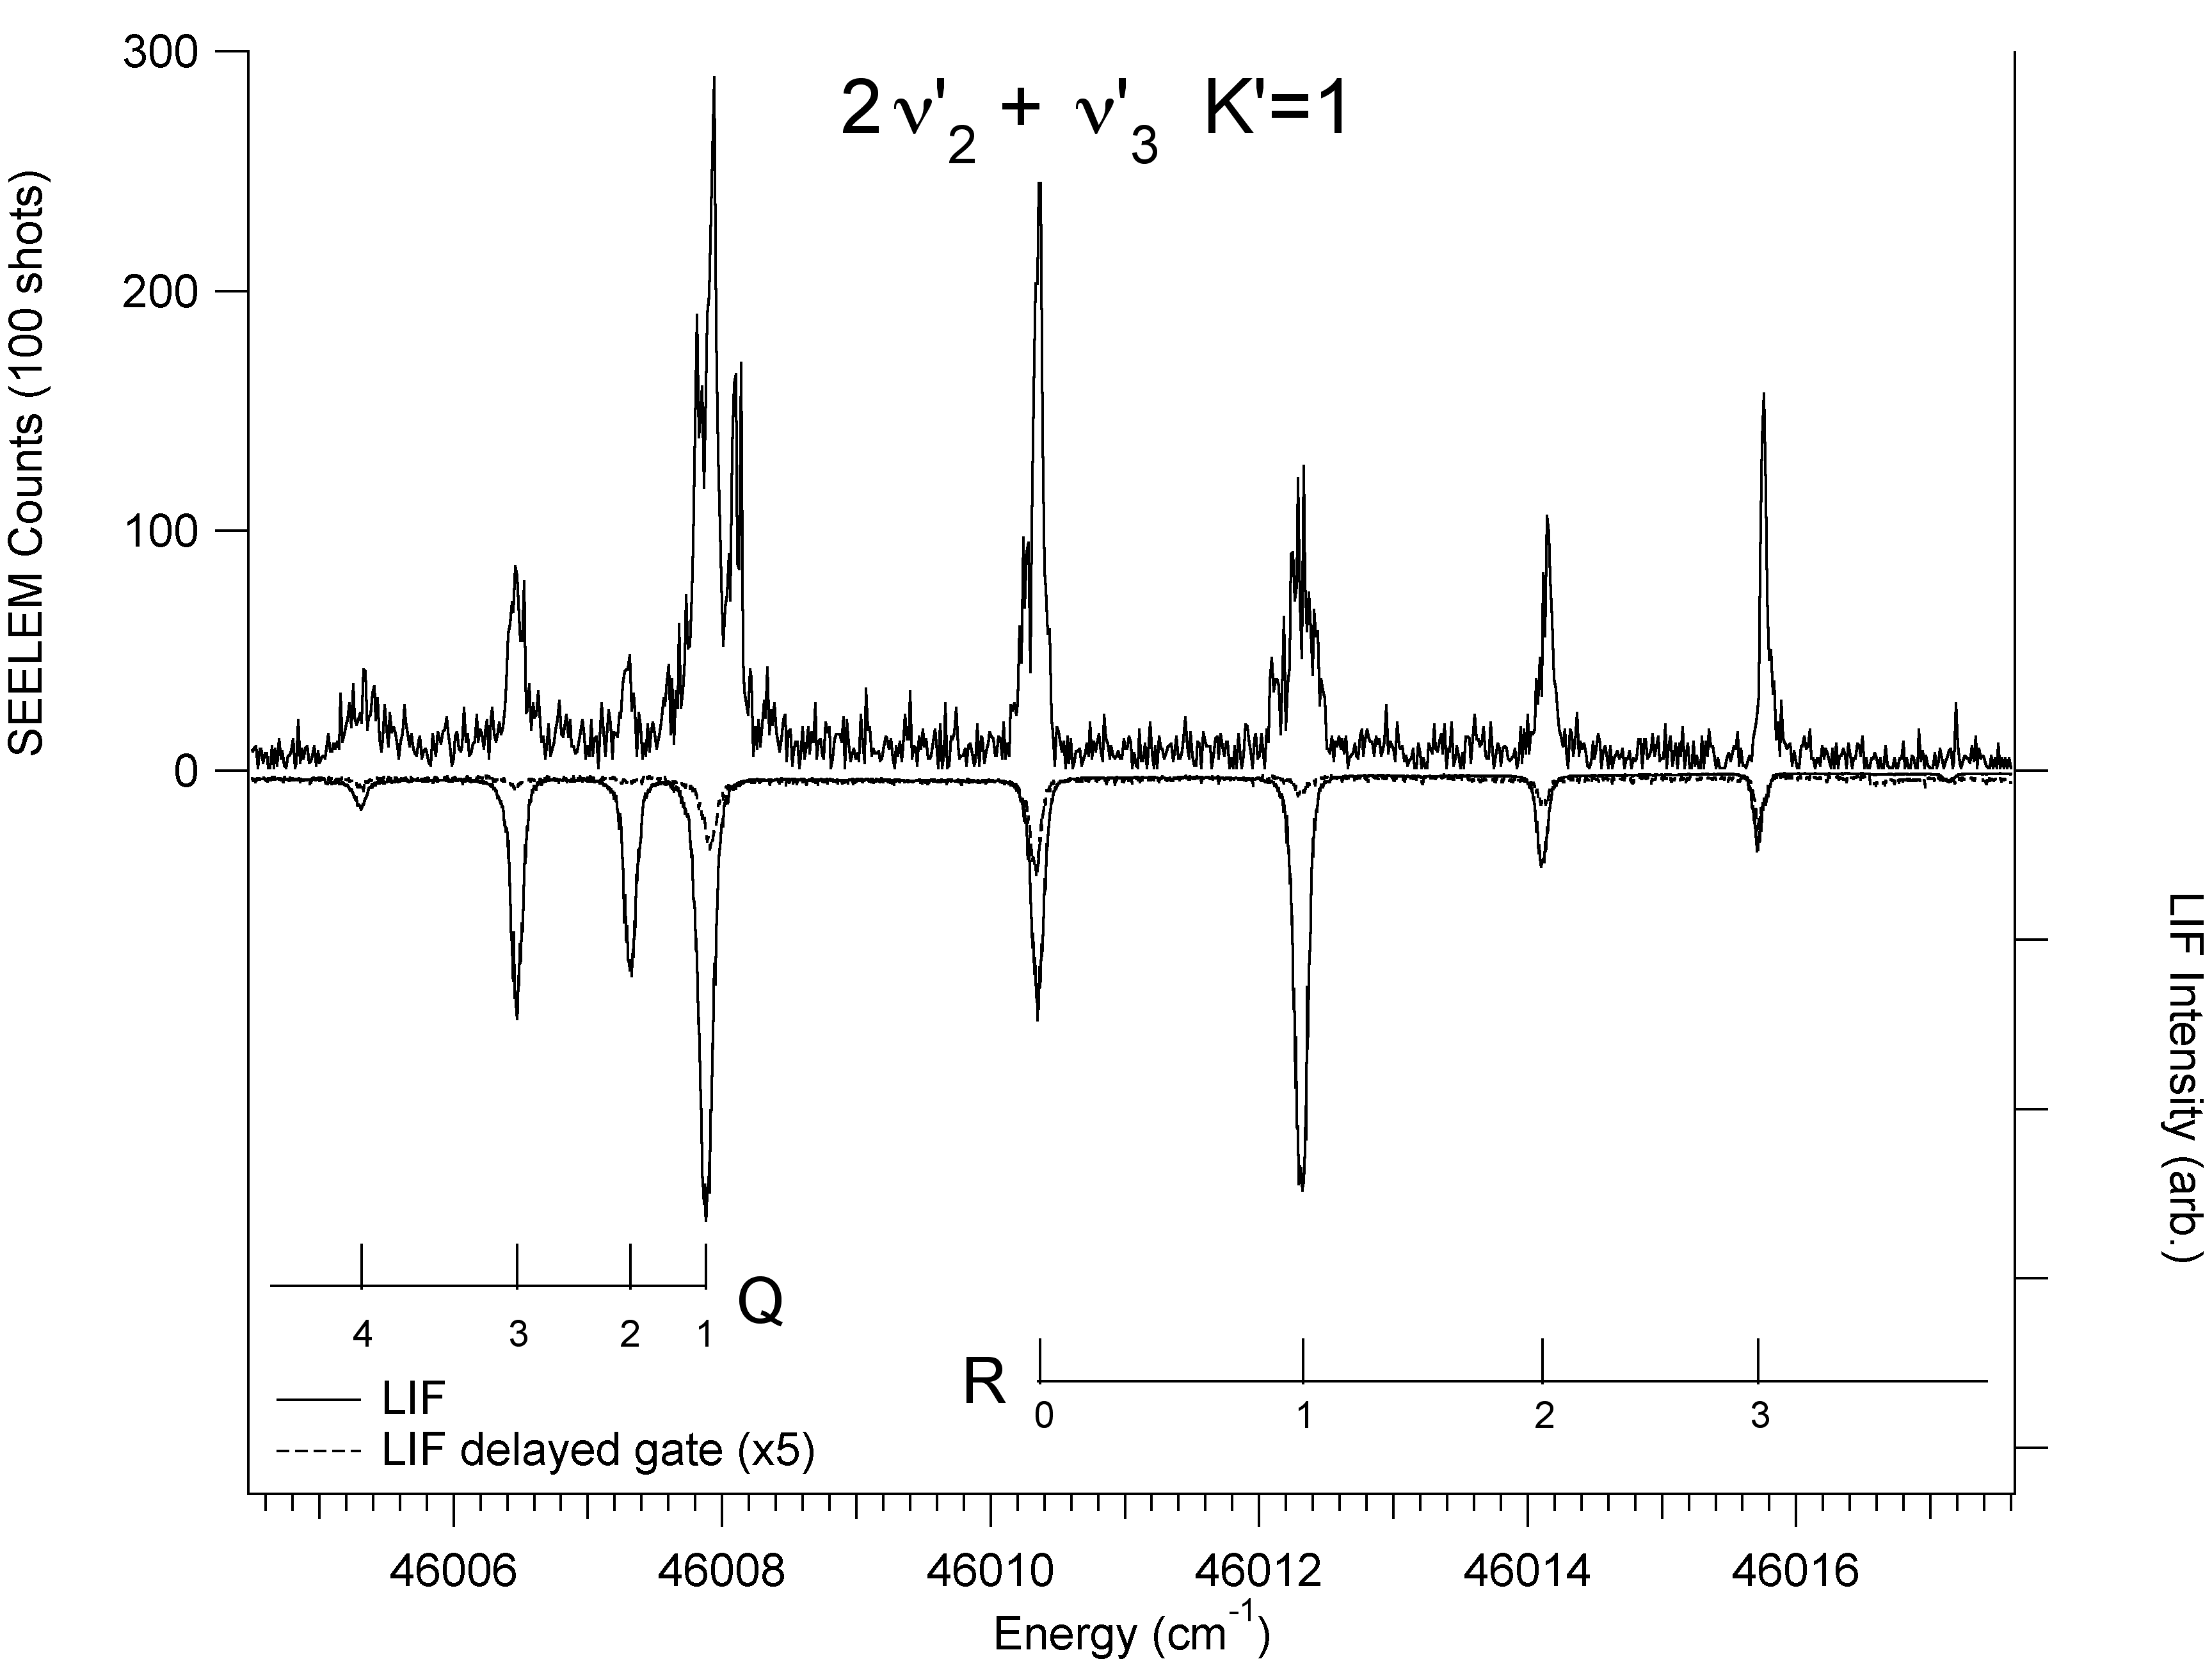
\includegraphics[width=7in,angle=90]{acetylene-2231-q4r3.png}
\end{figure}

\begin{figure}
  \caption{Dependence of the intensity-weighted center of gravity on
    delay for a series of rovibronic transitions, Q(1$-$4) (top), and
    R(0$-$3) (bottom), in the LIF spectrum of $2^23^1$ \Ka{1}.  The
    center of gravity for the Q(1) transition rapidly increases to its
    final value, where it matches the peak of the SEELEM distribution
    at 46007.87$+$0.03 \rcm.  For the R(0) transition, the center of
    gravity decreases at a nearly linear rate to 46010.35$-$0.3 \rcm.}
  \label{fig:2231-cog-delay}
  \centering
  \vspace{5mm}
  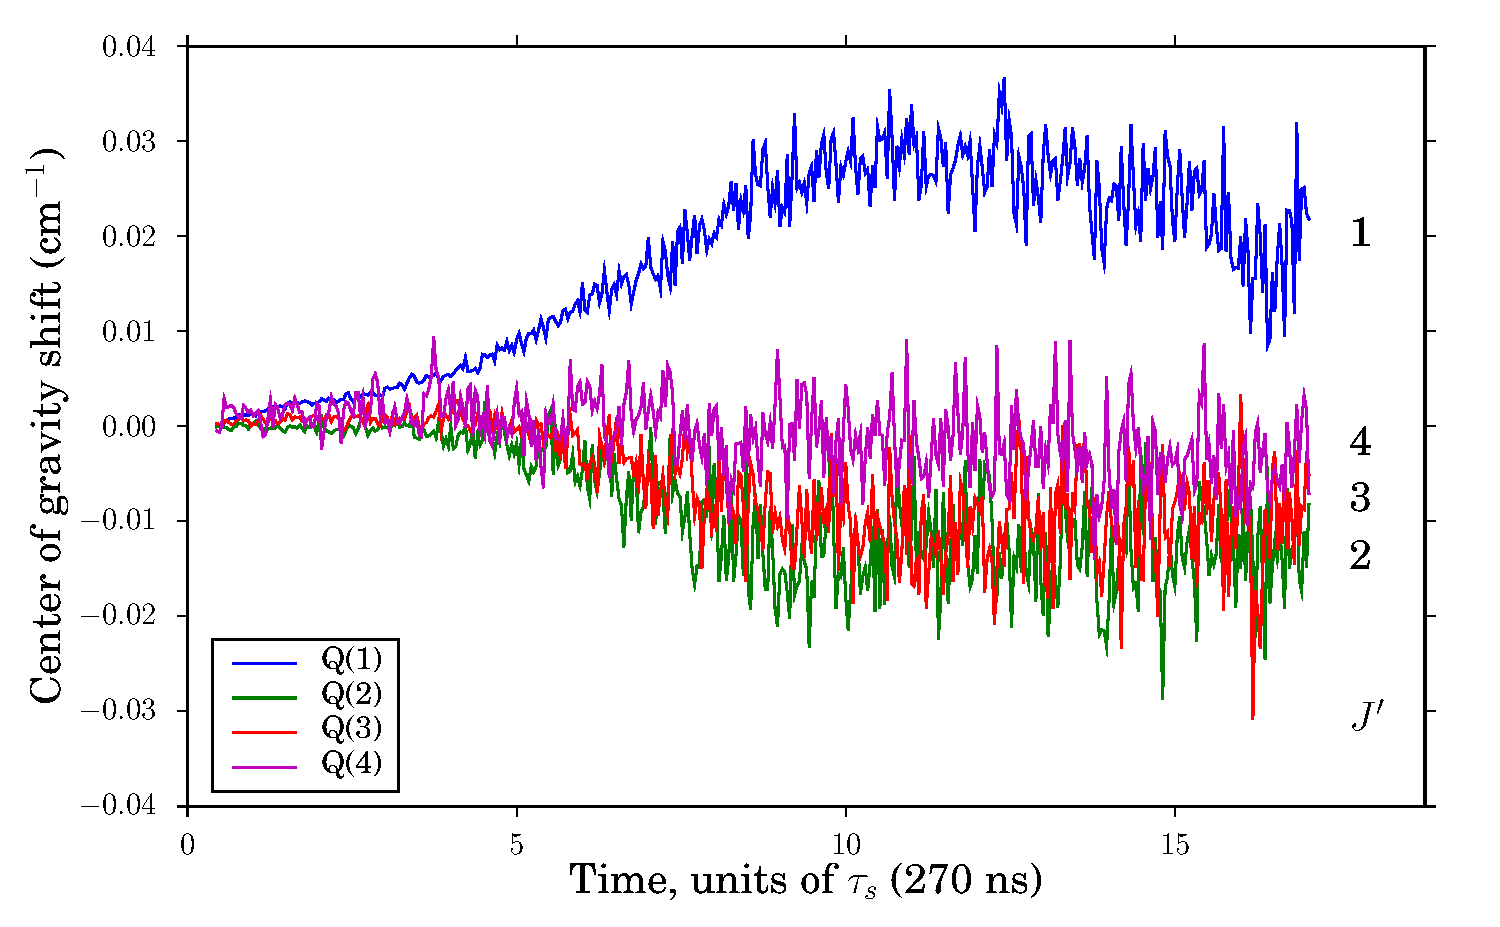
\includegraphics[width=6in]{2231-q1234-cog-delay.pdf}
  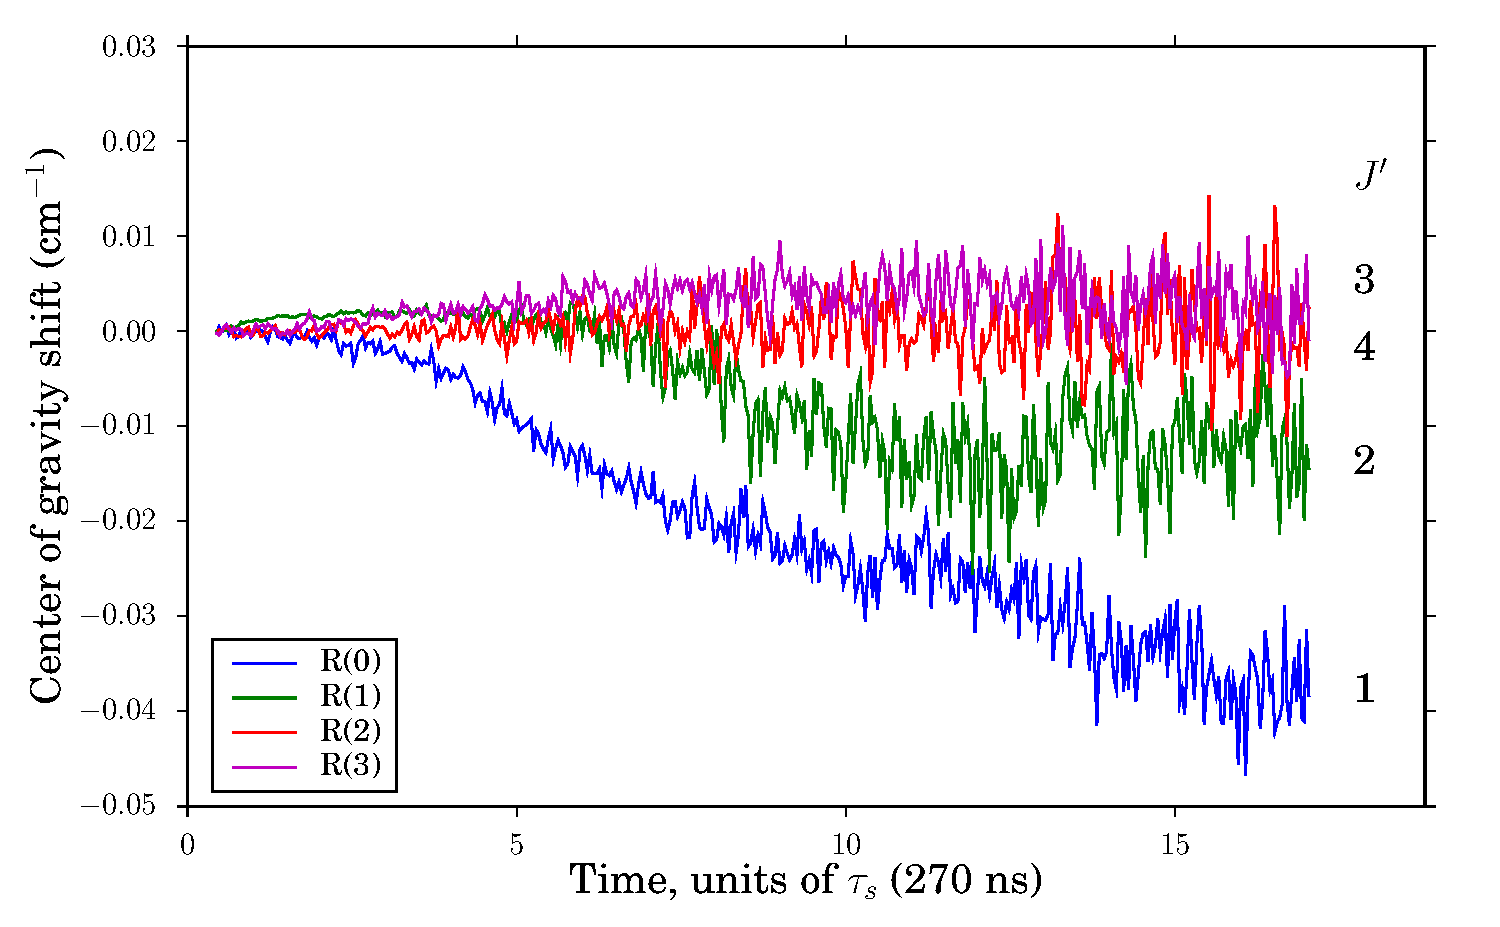
\includegraphics[width=6in]{2231-r0123-cog-delay.pdf}
\end{figure}

%%%%%%%%%%%%%%%%%%%%%%%%%%%%%%%%%%%%%%%%%%%%%%%%%%%%%%
%%
%% END OF 2^2 3^1 FIGURES
%%
%%%%%%%%%%%%%%%%%%%%%%%%%%%%%%%%%%%%%%%%%%%%%%%%%%%%%%

Although the $2^23^1$ \Ka{1} sublevel has the highest energy of the
four sublevels discussed in this study, it interacts most weakly with
the local manifold of $T_{1,2}$ levels.  This results from having only
one quantum of the $\nu_3$ vibration, which controls the overall
magnitude of $S_1 \sim T_3$ doorway matrix elements.

The spectrum of the $2^23^1$ \Ka{1} $\leftarrow$ $0_0$ subband is
shown in Figure \ref{fig:spectrum-2231}.  In addition to the overall
SEELEM:LIF intensity ratio, the small magnitude of $S_1 \sim T_3$
doorway matrix elements is indicated by the width of the SEELEM
intensity envelope surrounding each singlet transition.  This topic is
discussed at length in Chapter 2.  Briefly, the width of the SEELEM
spectrum is a measure of the energy range over which the singlet
level, through interaction with $T_3$ doorways, is able to lend
approximately 0.25\% fractional singlet character to eigenstates
within the local manifold of $T_{1,2}$ levels.  In the case of
$2^23^1$ \Ka{1}, the width of the SEELEM envelope surrounding each
singlet transition is on the order of 0.4 \rcm, much less than the
average spacing between rotational lines.  In the next section, we
will contrast this with the observed width of SEELEM intensity
envelopes in a strongly interacting subband.

% Using a formula
% derived in Chapter 2, the FWHM of the SEELEM spectrum can be related
% to the $S_1 \sim T_3$ doorway matrix element, $H_{S_1,T_3}$, and the
% average $T_3 \sim T_{1,2}$ matrix element, $\braket{H_{T_3,T_{1,2}}}$:
% \begin{equation}
%   \Delta E_{FWHM} = \frac{2\sqrt{2} \; \tau_s}
%                        {e \; \tau_{\text{flight}}}
%   \left \lvert
%     \frac{H_{S_1,T_3} \braket{H_{T_3,T_{1,2}}}}{\Delta E_{S_1,T_3}}
%   \right \rvert,
% \end{equation}
% where $\Delta E_{S_1,T_3}$ is the energy difference between the
% singlet level and the $T_3$ doorway, and $\tau_{\text{flight}}$ is the
% flight time in the SEELEM apparatus, about 310 \microsec.  Solving for
% the quantity $\lvert H_{S_1,T_3} \braket{H_{T_3,T_{1,2}}} / \Delta
% E_{S_1,T_3} \rvert$ and using the approximate FWHM of 0.4 \rcm, we
% find that
% \begin{equation}
% \end{equation}

The dependence of the intensity-weighted center of gravity for each
transition in $2^23^1$ \Ka{1} is shown in Figure
\ref{fig:2231-cog-delay}.  With the exception of the Q(1) and R(0)
transitions, the center of gravity does not shift by more than 0.02
\rcm\ from its initial position.  For a singlet level with such a
small spin-orbit matrix element with a doorway state, any small change
in center of gravity, which might arise from the effects of an
energetically distant $T_3$ level, is not expected to appear until
delay times in excess of $15\tau_s$.

\NOTE{Bob suggests interference effects here, but the basis for this
  is not clear to me.} The anomalous behavour of the center of gravity
for the Q(1) and R(0) transitions is once again evidence of a weak,
local $T_3$ perturbation at $J'=1$.  The upper states of the Q(1) and
R(0) transitions have the same $J'$, but differ in parity (being of
$f$- and $e$-symmetry, respectively).  The energy difference between
the \emph{e}- and \emph{f}-symmetry components is $\Delta
E_{e-f}=+0.13$ \rcm.  The perturbation in the \emph{e}-symmetry
singlet transition R(1) results in a shift to lower energy, with a
magnitude of approximately $-0.03$ \rcm, while the perturbation shifts the
\emph{f}-symmetry singlet level to lower energy, with a magnitude
of approximately $+0.03$ \rcm.  The splitting between the asymmetry
components of the $T_3$ perturber is therefore less than
$0.13-0.03-0.03=0.07$ \rcm at $J'=1$.  An asymmetry splitting of this
magnitude would be unusually small for a $T_3$ level with $K_T=1$.  As
a result, we conclude that the perturber is likely a level with
$K_T=2$.  Only one component of a $K_T=2$ level may interact with a
singlet level at $J'=1$, and that is the $F_3$ component, where
$N_T=J+1$.  An interaction with the $F_1$ or $F_2$ components would
require $N_T$ to be $0$ or $1$; these levels do not exist when
$K_T=2$.  Because the interaction occurs via the $F_2$ component of
the triplet level at $J'=1$, the rotationless energy of the triplet
level must be approximately $4B \simeq 4$ \rcm\ to the red of the
singlet level.

Again, the assignment of the $K_a$ quantum number for a $T_3$ level
observed in the spectrum has allowed us to infer its energy relative
to the singlet.  At $J'=2$, the nearest component of this weak $T_3$
perturber lies $2B \simeq 2$ \rcm\ above the singlet level.  The
resultant increase in squared energy denominator makes the
extra line $(2.0/0.03)^2 \simeq 4500$ times weaker at $J'=2$, and it
is not observed.

%
% Selection rules: Q   -> e-f
%                  P,R -> e-e, f-f
% 











\subsection{The $3^3$ \Ka{2} sublevel: spectral patterns in the
  presence of large $S_1 \sim T_3$ matrix elements}

% Spectrum:  Jan 22C, p.31,34 of 1/2007--3/2007 notebook.

%%%%%%%%%%%%%%%%%%%%%%%%%%%%%%%%%%%%%%%%%%%%%%%%%%%%%%
%%
%% INSERT 3^3 K^2 FIGURES HERE
%%
%%%%%%%%%%%%%%%%%%%%%%%%%%%%%%%%%%%%%%%%%%%%%%%%%%%%%%

\begin{figure}
  \caption{Simultaneously recorded SEELEM (upper trace) and LIF (lower
    trace) spectra of the $3^3$ \Ka{2} sublevel of the \astate\ state
    of \ce{C2H2}.  The LIF spectrum is integrated in two time regions:
    an early time window ($0.5\tau_s-2\tau_s$, solid trace) and a
    delayed time window ($10\tau_s-18\tau_s$, dashed trace).  The
    individual transitions each split into at least two strongly mixed
    components.  Although the energy splitting between the components
    is on the order of the experimental resolution, they are
    discernable via their different relative intenities in the early
    and delayed LIF spectra, which change the fluorescence lineshape.
    One splitting in the R(4) transition is barely resolved in this
    spectrum.  \TODO{Determine the assignment for the set of
      overlapping transitions.}}
  \label{fig:spectrum-33k2}
  \centering
  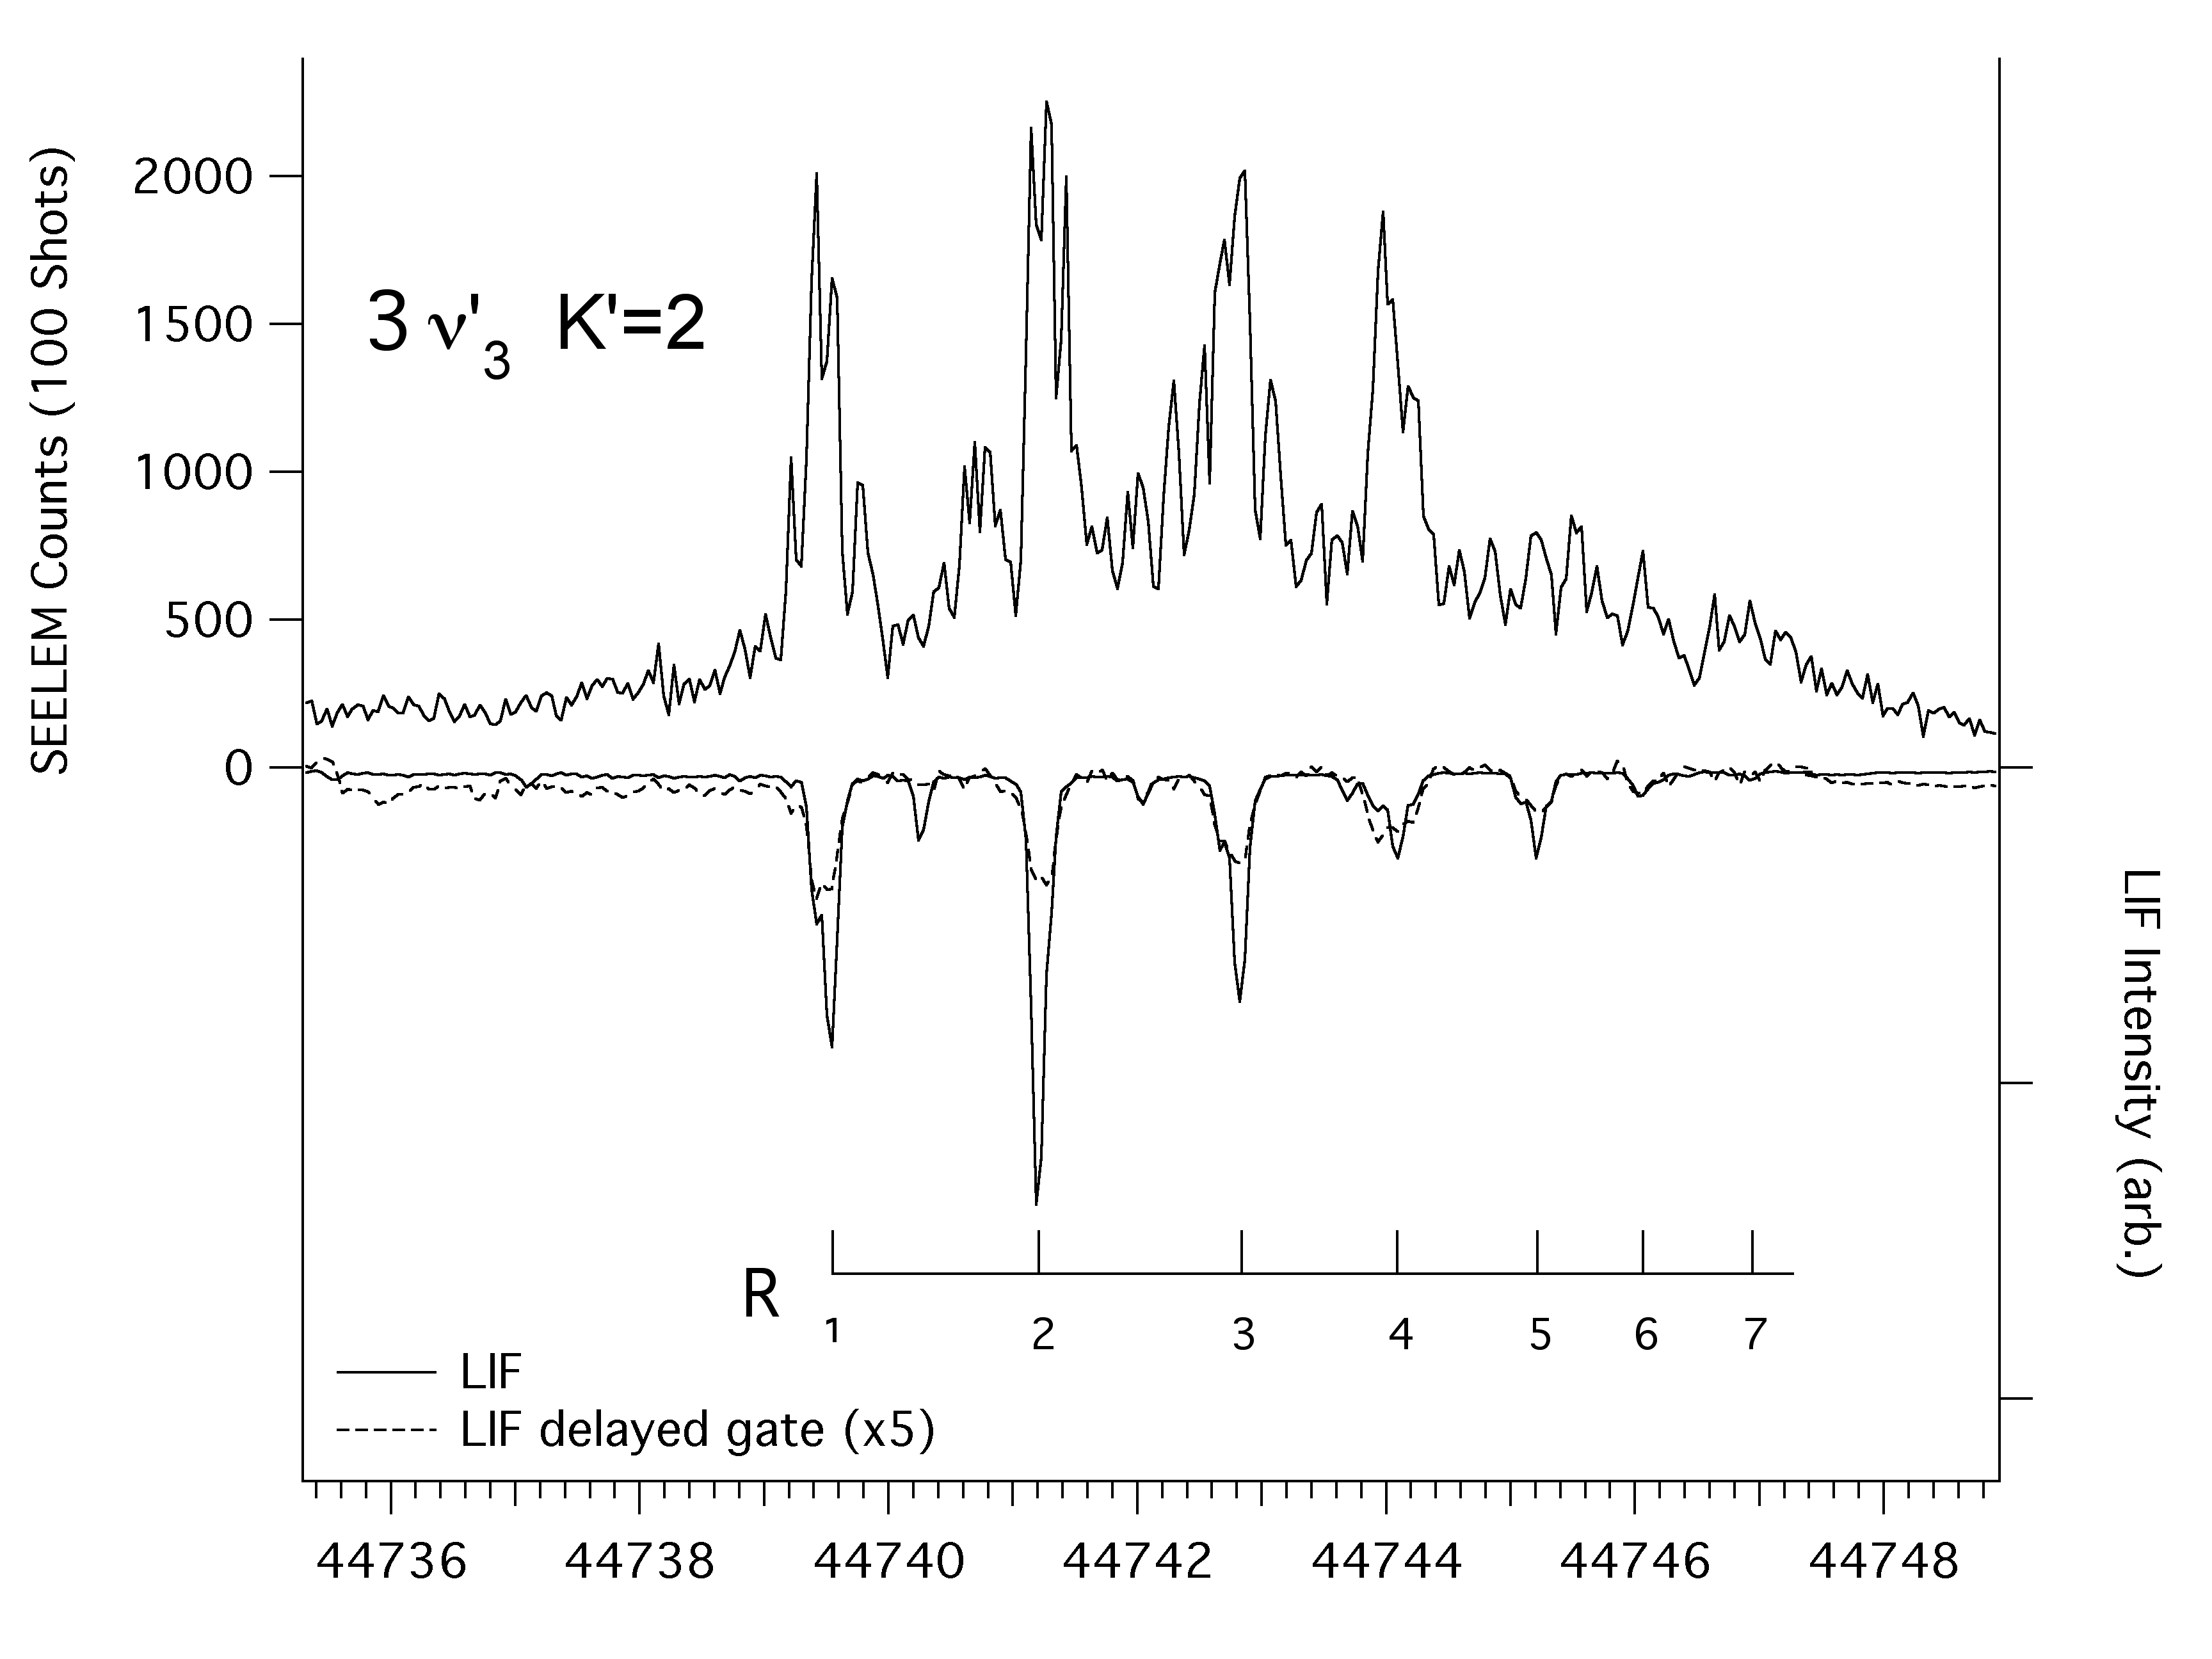
\includegraphics[width=7in,angle=90]{acetylene-33k2-r1r7.png}
\end{figure}

\begin{figure}
  \caption{Dependence of the intensity-weighted center of gravity on
    delay for a series of individually resolved transitions, R(1$-$7),
    in the LIF spectrum of the $3^3$ \Ka{2} sublevel.  The individual
    transitions have an overall bias toward lower energies at long
    delay times, indicating an interaction with a $T_3$ doorway level
    at lower energy.}
  \label{fig:33k2-cog-delay}
  \centering
  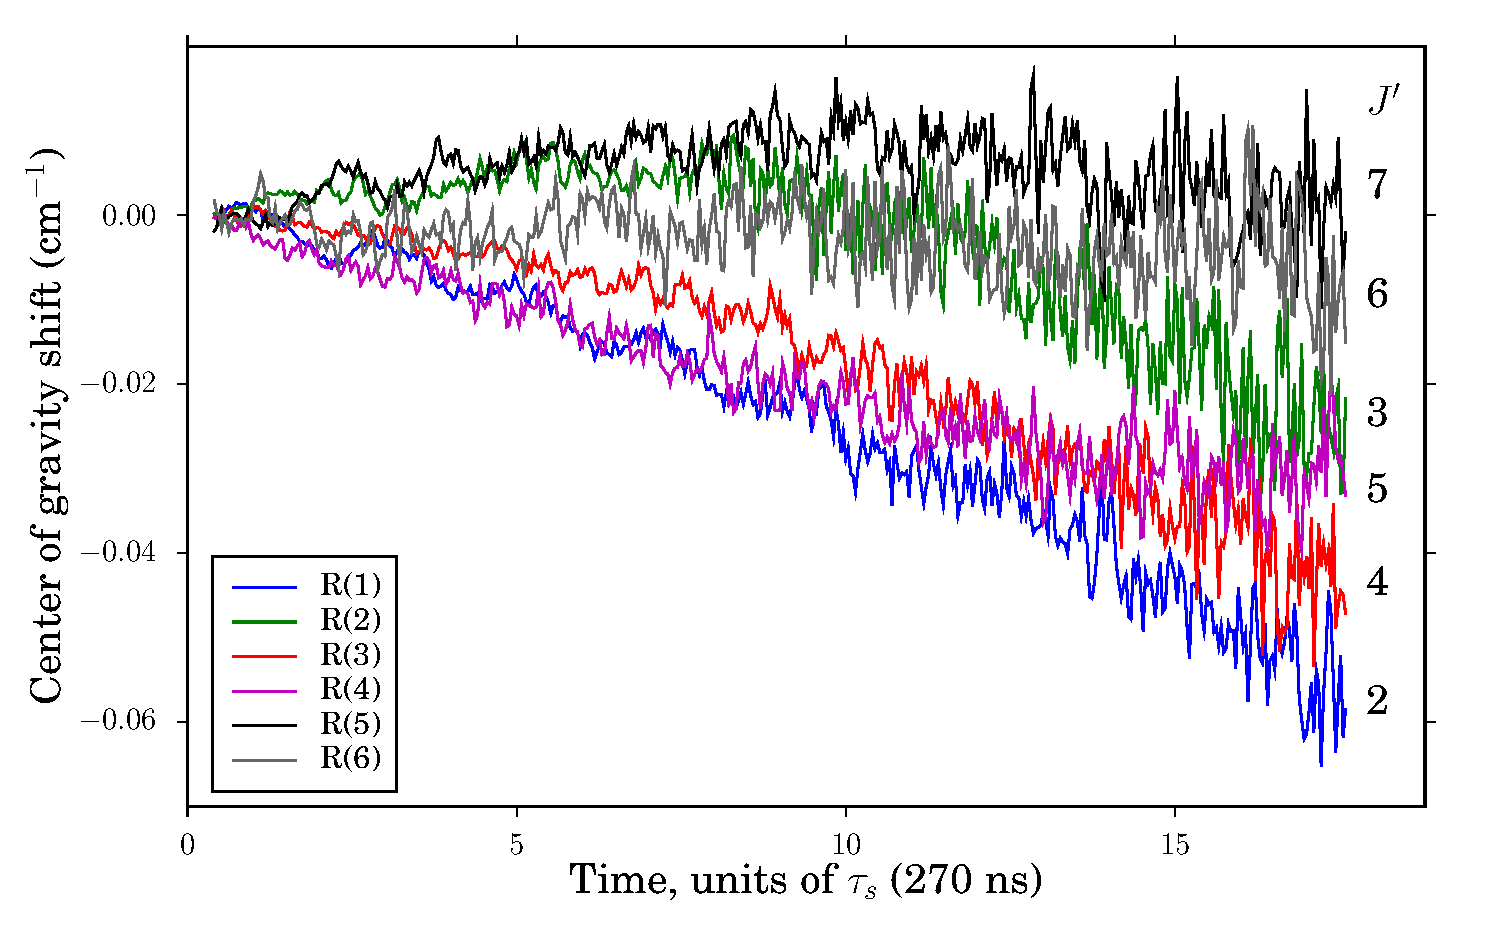
\includegraphics[width=6in]{33k2-r123456-cog-delay.pdf}
\end{figure}

%%%%%%%%%%%%%%%%%%%%%%%%%%%%%%%%%%%%%%%%%%%%%%%%%%%%%%
%%
%% END OF 3^3 K^2 FIGURES
%%
%%%%%%%%%%%%%%%%%%%%%%%%%%%%%%%%%%%%%%%%%%%%%%%%%%%%%%

The $3^3$ \Ka{2} sublevel is the higher-energy sibling of $3^3$
\Ka{1}, which has been studied in great detail due to a
perturbation by a $T_3$ doorway level with matrix element $\simeq
0.1$ \rcm.  The $T_3$ pertuber observed in $3^3$ \Ka{1} has been
assigned as the $F_2$ component of $K_T=1$, because 
%\begin{inparaenum}[\itshape a\upshape)]
%\item 
it tunes slowly with energy relative to $S_1$,
%\item 
it interacts with both parities of the singlet, and
%\item 
the perturbation is present at $J'=1$
%\end{inparaenum}
\cite{mishra04}.  It has been suggested that the $K_T=0$ sublevel of
this perturber is responsible for the large Zeeman anticrossing
observed in $3^3$ \Ka{0} \cite{thom07, dupre93}.  To account for this,
the $A$-rotational constant of the perturbing $T_3$ level would have
to closely match the $A$-rotational constant for the singlet level.  However, it is
unlikely that an energetic near match in the $K=0$ and $1$
sublevels, separated by $1A \simeq 15$ \rcm, will extend to $K=2$,
which is $3A \simeq 45$ \rcm\ higher in energy.  In the absence of a
local $T_3$ perturbation, the $3^3$ \Ka{2} sublevel provides an
excellent opportunity to look examine a singlet sublevel which is
known to be capable of large vibrational overlap with $T_3$ levels.

The $3^3$ \Ka{2} sublevel is not accessible from the ground state of
acetylene due to $K' - \ell" = \pm 1$ selection rules.  However, the
spectrum of the $3^3$ \Ka{2} $\leftarrow$ $4_1$ hot band transition
was obtained in our apparatus without heating the nozzle.  The
simultaneously recorded SEELEM/LIF spectrum of the R-branch of this
transition is shown in Figure \ref{fig:spectrum-33k2}.  Another
interloping band is present in the spectrum with low intensity,
giving rise to the weak lines at 44740.3, 44742.2, and 44743.6 \rcm.
No intensity alternation is present in the rotational series, as
expected for a band that originates from the $4_1$ vibrational level
of the ground electronic state.

Evidence of strong mixing with the local manifold of $T_{1,2}$ levels
is present in both the SEELEM and LIF detection channels.  The SEELEM
intensity envelope surrounding each singlet transition exceeds the
spacing between adjacent rotational lines, about 1.5 \rcm at low $J'$.
This is at least 4 times the width observed for the transitions in
$2^23^1$ \Ka{1}, which contains only one quantum of excitation in
$\nu_3$.  The increased width of the local SEELEM intensity envelope
has the effect of creating an envelope of SEELEM intensity that
extends across the entire spectrum.  This effect is also observed in
the $3^3$ \Ka{1} $\leftarrow$ $0_0$ spectrum (see reference
\cite{humphrey97}, for example).  

However, we observe no large, systematic splittings at adjacent
rotational levels of $3^3$ \Ka{2}, which would result from a level
crossing with the $F_2$ component of a near-degenerate $T_3$ doorway
vibrational level, as in $3^3$ \Ka{1} \cite{mishra04}.  Instead,
narrow line splittings on the order of 0.05 \rcm\ are evident in the
LIF spectrum of each transition, even in the early time-gated LIF
spectrum.  Although most of the line splittings are slightly smaller
than the laser resolution, the individual components have different
fractional $S_1$ character, and hence different lifetimes.  This
produes different relative intensities in the early and delayed LIF
spectra, which permits the splittings to be observed by comparing the
spectra.  Two of three strong components are just resolved in the
early LIF spectrum of the R(4) transition.  In contrast to this
strongly $S_1 \sim T_3$ mixed sublevel, the weakly mixed $2^23^1$
\Ka{1} sublevel contains no such splittings.

The dependence of the intensity-weighted center of gravity for each
transition in $3^3$ \Ka{2} is shown in Figure
\ref{fig:33k2-cog-delay}.  The transitions display an overall bias
toward lower energy, indicating the presence of a $T_3$ doorway level
to lower energy.  The $F_3$ components of such a doorway level would
approach the singlet level from below at a rate of $2B$ per $J'$,
while the $F_2$ components would remain energetically distant and the
$F_1$ components would rapidly tune away.  That no crossing is
observed by at least $J'=6$ means that the doorway must lie at least
$6\times2B + 2B \simeq 14$ \rcm\ lower in energy than the singlet
level.

The center of gravity vs. gate delay changes with the greatest
magnitude for the $J'=2$ rotational level, and the magnitude of shift
generally decreases with $J'$.  However, if the $F_3$ component of the
doorway level is rapidly approaching the singlet, the overall mixing
angle is expected to increase in magnitude.  Why does the magnitude of
the change in center of gravity not also increase?  This paradox is
explained by the large fractional singlet character in nominal
$T_{1,2}$ levels, which is induced by strong mixing with the doorway
level.  As several components of nominal $T_{1,2}$ electronic
character borrow more intensity, their lifetime decreases.  As the
nominal singlet level lends out more fractional character, its
lifetime increases.  The result is a lack of contrast between the
intensities of the nominal singlet and nominal triplet eigenstates as
a function of delay time, resulting in smaller changes in the
intensity-weighted center of gravity.

However, evidence for the approach toward $S_1$ of energetically
distant $T_3$ doorway levels is still available from the spectrum.
The most reliable indicator is a comparison of band-integrated center
of gravity of the early LIF spectrum vs. the SEELEM spectrum.  We
discuss this in the following section.

\subsection{Evidence for energetically distant $T_3$ doorway levels in
  band-integrated center of gravity}

%%%%%%%%%%%%%%%%%%%%%%%%%%%%%%%%%%%%%%%%%%%%%%%%%%%%%%
%%
%% INSERT CENTER OF GRAVITY TABLE HERE
%%
%%%%%%%%%%%%%%%%%%%%%%%%%%%%%%%%%%%%%%%%%%%%%%%%%%%%%%

\begin{table}[p]
  \caption{Band-integrated center of gravity measurements from
    simultaneously recorded SEELEM/LIF spectra of \astate\ acetylene.
    The SEELEM$-$LIF center of gravity is offset to lower energy for
    Q-branch measurements and offset to higher energy for R-branch measurements, 
    indicating an overall increase in relative SEELEM:LIF intensity
    with $J'$.  Such $J'$-dependent behavior is predicted in the
    presence of energetically distant $T_3$ doorway levels.}
  \label{table:integrated-cog-shifts}

  \centering
        \begin{tabular}{lllll}
        \\[1cm]
        \multicolumn{3}{l}{Q-branch measurements} \\
        \toprule
        Level & Integration region & \multicolumn{2}{l}{Center of gravity} & Offset \\
        \cmidrule{3-5}
        & & LIF & SEELEM & SEELEM$-$LIF \\
        \midrule
        $\nu'_2+2\nu'_3$ & 45671.75$-$76.30 & 45674.60 & 45674.09 & $-0.51$ \\
        $2\nu'_2+\nu'_3$ & 46004.50$-$08.50 & 46007.29 & 46007.23 & $-0.06$ \\
        $2\nu'_3+2\nu'_4$ & 45807.30$-$11.00 & 45810.09 & 45809.72 & $-0.37$ \\
        \bottomrule
        \end{tabular}

        \begin{tabular}{lllll}
        \\[1cm]
        \multicolumn{3}{l}{R-branch measurements} \\
        \toprule
        Level & Integration region & \multicolumn{2}{l}{Center of gravity} & Offset \\
        \cmidrule{3-5}
        & & LIF & SEELEM & SEELEM$-$LIF \\
        \midrule
        $2\nu'_2+\nu'_3$ & 46009.50$-$16.50 & 46012.11 & 46012.49 & $+0.38$ \\
        $3\nu'_3 \:\; K'\!=\!2$ & 44738.50$-$47.50 & 44741.79 & 44742.67 & $+0.88$ \\
        $2\nu'_3+2\nu'_4$ & 45812.00$-$20.50 & 45814.67 & 45815.57 & $+0.89$ \\
        \bottomrule
        \end{tabular}
\end{table}

%%%%%%%%%%%%%%%%%%%%%%%%%%%%%%%%%%%%%%%%%%%%%%%%%%%%%%
%%
%% END CENTER OF GRAVITY TABLE
%%
%%%%%%%%%%%%%%%%%%%%%%%%%%%%%%%%%%%%%%%%%%%%%%%%%%%%%%

\NOTE{Just the table for now.}





























\section{Conclusion}

The mechanism of doorway-mediated coupling by an energetically distant
$T_3$ level skews the coupling to the local $T_{1,2}$ states that
appear in the SEELEM spectrum, resulting in a center of gravity shift
between the LIF and SEELEM spectra.  Additionally, when viewed in
successive time windows, the center of gravity of the LIF spectrum
exhibits evolution toward the limiting behavior exhibited in the
SEELEM spectrum.  A simple model can be used to show that strong
coupling between the singlet level and the mediating $T_3$ level
causes a gradual shift in the center of gravity, while weak coupling
to the mediating level induces a more delayed and rapid shift in the
center of gravity, with respect to the $S_1$ lifetime.

Rotational selection rules for $S_1 \sim T_3$ spin-orbit coupling give
rise to $J$-dependent effects in the LIF/SEELEM spectrum.  As $J$
increases, the $\Delta N$= +1 or -1 components of any distant $T_3$
level approach the singlet at a rate $d\Delta E / dJ$ of approximately
$2B_T$ ($\sim$2 \rcm\ per $J$).  In the spectrum, the result is a
shift in the LIF-SEELEM center of gravity when integrated across an
entire branch of transitions.  The effect not only leads to strong
$J$-dependent changes in the patterns of $T_3$-mediated coupling, but
also ensures detection and assignment of $S_1 \sim T_3$ level
crossings at relatively low values of $J$.

% \POINT{The LIF/SEELEM spectra for the progression of $2^n3^m$ levels
%   shows the expected trends for strong coupling.}

\POINT{For every $S_1$ vibrational level, a $T_3$ doorway level is
  rapidly approaching with $J$.}  Because of this, further LIF/SEELEM
spectroscopy of the acetylene \AtoX\ transition will be fruitful and
informative.  We highlight some candidates for future investigation.
\begin{enumerate}
\item Levels which exhibit long lifetimes or quantum beats in the LIF
  spectrum
\item levels with unassigned perturbations or splittings,
\item other $3^2B^2$ polyad members
\item other $K$-sublevels of the Franck-Condon active levels studied
  here.  
\end{enumerate}
\TODO{Specify candidate bands specifically, give energies.}

The appearance of population quantum beats in the spectrum indicates a
splitting on the order of 80 MHz or less.  Quantum beat waveforms
follow a well-defined analytical expression, and an analysis of
quantum beats determines both the matrix element and zero-order energy
spacing of the levels involved.  The matrix elements gained from an
analysis of zero-field quantum beats in the acetylene spectrum can
serve as a probe of the magnitude of local matrix elements between the
nominal $S_1$ bright state and neighboring $T_{1,2}$ dark states.
Furthermore, the study of Zeeman quantum beats at low magnetic fields
can provide a method for distinguishing between triplet perturbations
and perturbations from other singlet levels, such as $S_1$ levels
which are localized in the \emph{cis} geometry of the \astate\ state.

\bibliography{master} 
\bibliographystyle{plain}
\end{document}
% LocalWords:  redshifted blueshifted sublevel pdf png



President's Report:

The T_3 electronic state is peculiar among the valence states of
acetylene due to its out-of-plane equilibrium geometry. One of the
most interesting unsolved problems in the intersystem crossing of
acetylene is the role of the non-symmetric in- and out-of-plane S_1
bending modes (\nu_4 and \nu_6) in promoting coupling to the nonplanar
T_3 state.  To investigate this issue, we have used an IR-UV-Double
Resonance technique to record simultaneous LIF/SEELEM spectra of the
3^3 4^1 K=0 and 3^3 6^1 K=0 levels.  This method allows us to record
the spectrum of weakly coupled T_1,2 levels without overlap from
adjacent rotational transitions.

[Additionally, we have used a polarization technique in tandem with
IRUVDR to record the spectrum of the rotationless level in 3^3 6^1
K=0.  Due to spin-orbit selection rules, only triplet levels having
K_T = J_T = N_T = 0 may appear in the spectrum -- thus, the local
T_1,2 level density may be obtained from a direct count of SEELEM
transitions.]


That should be K_T = J_T = 0 and N_T = 1...my bad. For a K=0 triplet
level in Hund's case (b),

N            J

  ---------- 3
2 ---------- 2
  ---------- 1


  ---------- 2
1 ---------- 1
  ---------- 0  ***


0 ---------- 1

--Kyle



The total spin-orbit matrix element between a rovibronic level of S_1
and a level of T_3 is the product of an electronic factor, a
vibrational overlap factor, and a rotational factor (arising from
angular momentum coupling laws).

OK, these are kind of hairy, but hold on before you start to panic.
As it turns out, the energy differences between levels of S_1 and T_3
vary much more rapidly than the rotational factors.  This is due to
the spin-orbit selection rule of \Delta_N = 0, +1, -1.

Take a look at this plot: It shows the relative energies of the three
triplet rotational components that are connected to singlet level: F_1
(\Delta_N = -1), F_2 (\Delta_N = 0), and F_3 (\Delta_N = +1).  This
plot is made in the approximation that the singlet and triplet
B-values are nearly equal.  Imagine placing a singlet level at some
energy on the plot - the energy of the singlet could be represented by
a horizontal line.  If the singlet is very close to zero, the F_2
component varies slowly with rotation and the F_1,2 components rapidly
speed away.  Essentially, only the F_2 component matters when J>1.

If the singlet is not located close to zero, EITHER the F_1 or the F_3
component of the triplet is rapidly approaching.  The triplet
component approaches with a rate of about 2 cm-1 per rotational
quantum number. According to Ryan and Bryan's calculations, the
<electronic*vibrational> spin-orbit matrix elements between S_1 and
T_3 max out at about 0.1 cm-1. The rotational factor only reduces this
value.  Compared to the matrix element, an energy difference of 2 cm-1
per J is huge!

I believe that strongly coupled, mediating T_3 levels will make
themselves known at several values of J through this
energy-denominator effect.  I think this is what we observe in our 3^3
K=2 data.  Weakly coupled T_3 levels should appear as perturbations at
a single J, and then immediately disappear, because their matrix
elements are much, much less than 2 cm-1. This means that weak triplet
perturbations should be _common_, and it means that we should be able
to infer their approximate energy from the value of J which is
perturbed in the singlet, i.e. + or - (J*2*B).

This means that further SEELEM spectroscopy of the S_1 state should be
fruitful and informative.  I hope you are all totally stoked!  I'll
discuss the experimental consequences and possibilities in a later
email.

--Kyle
